\documentclass[journal,10pt,romanappendices]{IEEEtai}
\usepackage[utf8]{inputenc}
\usepackage[T1]{fontenc}
\usepackage{amsmath,amssymb,amsthm,mathtools}
\usepackage{booktabs,graphicx,microtype,placeins,array,needspace}
\usepackage[numbers,sort&compress]{natbib}
\usepackage{xurl,hyperref}
\usepackage{xr}
\newcommand{\ArticleTitle}{A Two-Grid Characterization of Euler Sampling Accuracy in Flow Matching}
\hypersetup{pdftitle={A Two-Grid Characterization of Euler Sampling Accuracy in Flow Matching},pdfauthor={Dev D. Goyal},pdflang={en-US},colorlinks=true,linkcolor=blue,citecolor=blue,urlcolor=blue}
\newtheorem{theorem}{Theorem}
\newtheorem{proposition}[theorem]{Proposition}
\newtheorem{lemma}[theorem]{Lemma}
\newtheorem{corollary}[theorem]{Corollary}
\theoremstyle{definition}
\newtheorem{definition}{Definition}
\newcommand{\R}{\mathbb R}
\newcommand{\E}{\mathbb E}
\newcommand{\tr}{\operatorname{tr}}
\newcommand{\Law}{\operatorname{Law}}
\newcommand{\dd}{\,\mathrm d}

\newcommand{\AIcitations}{\citep{openai_chatgpt,openai_codex,anthropic_claude,anthropic_claude_fable}}
\newcommand{\AIassistance}{\footnote{AI assistance for this section is disclosed in the acknowledgment~\AIcitations.}}

\newcommand{\IntroExactFlow}{$1.02$}
\newcommand{\RiskMeshThreshold}{1.3\times10^{-14}}
\newcommand{\RiskStepCount}{7.7\times10^{13}}
\newcommand{\ScalarCfmArgminEight}{0}
\newcommand{\ScalarCfmArgminLast}{3}
\newcommand{\ScalarCfmArgminSixteen}{0}
\newcommand{\ScalarCfmBias}{0.091}
\newcommand{\ScalarCfmBiasMax}{0.195}
\newcommand{\ScalarCfmBiasMin}{0.023}
\newcommand{\ScalarCfmEight}{0.174}
\newcommand{\ScalarCfmFromSixteenIncreaseLarge}{0}
\newcommand{\ScalarCfmFromSixteenIncreaseSixtyFour}{0}
\newcommand{\ScalarCfmFromSixteenWilcoxonLarge}{0.002}
\newcommand{\ScalarCfmFromSixteenWilcoxonSixtyFour}{0.002}
\newcommand{\ScalarCfmIncreaseLarge}{0}
\newcommand{\ScalarCfmIncreaseSixteen}{0}
\newcommand{\ScalarCfmIncreaseSixtyFour}{0}
\newcommand{\ScalarCfmLarge}{0.090}
\newcommand{\ScalarCfmOwnEight}{0.153}
\newcommand{\ScalarCfmOwnLarge}{0.005}
\newcommand{\ScalarCfmPairCoarse}{0.174}
\newcommand{\ScalarCfmPairFine}{0.115}
\newcommand{\ScalarCfmSdMax}{0.063}
\newcommand{\ScalarCfmSixteen}{0.115}
\newcommand{\ScalarCfmSixtyFour}{0.090}
\newcommand{\ScalarCfmWilcoxonLarge}{0.002}
\newcommand{\ScalarCfmWilcoxonSixteen}{0.002}
\newcommand{\ScalarCfmWilcoxonSixtyFour}{0.002}
\newcommand{\ScalarExactBias}{0.000}
\newcommand{\ScalarExactEight}{0.151}
\newcommand{\ScalarExactLarge}{0.005}
\newcommand{\ScalarExactOwnEight}{0.151}
\newcommand{\ScalarExactOwnLarge}{0.005}
\newcommand{\ScalarExactSdMax}{0.000}
\newcommand{\ScalarExactSixteen}{0.077}
\newcommand{\ScalarExactSixtyFour}{0.020}
\newcommand{\ScalarModelCount}{30}
\newcommand{\ScalarOneArgminEight}{6}
\newcommand{\ScalarOneArgminLast}{0}
\newcommand{\ScalarOneArgminSixteen}{4}
\newcommand{\ScalarOneBias}{0.125}
\newcommand{\ScalarOneBiasMax}{0.193}
\newcommand{\ScalarOneBiasMin}{0.084}
\newcommand{\ScalarOneEight}{0.085}
\newcommand{\ScalarOneFromSixteenIncreaseLarge}{10}
\newcommand{\ScalarOneFromSixteenIncreaseSixtyFour}{10}
\newcommand{\ScalarOneFromSixteenWilcoxonLarge}{0.002}
\newcommand{\ScalarOneFromSixteenWilcoxonSixtyFour}{0.002}
\newcommand{\ScalarOneGridFactor}{1.4}
\newcommand{\ScalarOneIncreaseLarge}{10}
\newcommand{\ScalarOneIncreaseSixteen}{6}
\newcommand{\ScalarOneIncreaseSixtyFour}{10}
\newcommand{\ScalarOneLarge}{0.122}
\newcommand{\ScalarOneOwnEight}{0.125}
\newcommand{\ScalarOneOwnLarge}{0.004}
\newcommand{\ScalarOnePairCoarse}{0.085}
\newcommand{\ScalarOnePairFine}{0.084}
\newcommand{\ScalarOneSdMax}{0.041}
\newcommand{\ScalarOneSixteen}{0.084}
\newcommand{\ScalarOneSixtyFour}{0.113}
\newcommand{\ScalarOneWilcoxonLarge}{0.002}
\newcommand{\ScalarOneWilcoxonSixteen}{0.695}
\newcommand{\ScalarOneWilcoxonSixtyFour}{0.002}
\newcommand{\ScalarTwoArgminEight}{0}
\newcommand{\ScalarTwoArgminLast}{0}
\newcommand{\ScalarTwoArgminSixteen}{9}
\newcommand{\ScalarTwoBias}{0.096}
\newcommand{\ScalarTwoBiasMax}{0.127}
\newcommand{\ScalarTwoBiasMin}{0.062}
\newcommand{\ScalarTwoEight}{0.092}
\newcommand{\ScalarTwoFromSixteenIncreaseLarge}{10}
\newcommand{\ScalarTwoFromSixteenIncreaseSixtyFour}{10}
\newcommand{\ScalarTwoFromSixteenWilcoxonLarge}{0.002}
\newcommand{\ScalarTwoFromSixteenWilcoxonSixtyFour}{0.002}
\newcommand{\ScalarTwoIncreaseLarge}{5}
\newcommand{\ScalarTwoIncreaseSixteen}{0}
\newcommand{\ScalarTwoIncreaseSixtyFour}{4}
\newcommand{\ScalarTwoLarge}{0.093}
\newcommand{\ScalarTwoOwnEight}{0.126}
\newcommand{\ScalarTwoOwnLarge}{0.004}
\newcommand{\ScalarTwoPairCoarse}{0.092}
\newcommand{\ScalarTwoPairFine}{0.069}
\newcommand{\ScalarTwoSdMax}{0.026}
\newcommand{\ScalarTwoSixteen}{0.069}
\newcommand{\ScalarTwoSixtyFour}{0.085}
\newcommand{\ScalarTwoWilcoxonLarge}{0.846}
\newcommand{\ScalarTwoWilcoxonSixteen}{0.002}
\newcommand{\ScalarTwoWilcoxonSixtyFour}{0.375}
\newcommand{\VarMediumAllSix}{0.0}
\newcommand{\VarMediumAnySix}{7}
\newcommand{\VarMediumCfmFractionMax}{0}
\newcommand{\VarMediumChangeMean}{-0.015}
\newcommand{\VarMediumChangeSd}{0.005}
\newcommand{\VarMediumFractionMax}{7}
\newcommand{\VarMediumFractionMin}{0}
\newcommand{\VarMediumGridLongFraction}{100}
\newcommand{\VarMediumGridLongMean}{0.014}
\newcommand{\VarMediumLongOneA}{100}
\newcommand{\VarMediumLongOneB}{30}
\newcommand{\VarMediumLongOneC}{77}
\newcommand{\VarMediumLongTwoA}{33}
\newcommand{\VarMediumLongTwoB}{7}
\newcommand{\VarMediumLongTwoC}{20}
\newcommand{\VarMediumSets}{30}
\newcommand{\VarSetCount}{230}
\newcommand{\VarSmallAllSix}{2.5}
\newcommand{\VarSmallAnySix}{43}
\newcommand{\VarSmallCfmFractionMax}{0}
\newcommand{\VarSmallChangeMean}{-0.011}
\newcommand{\VarSmallChangeSd}{0.014}
\newcommand{\VarSmallFractionMax}{38}
\newcommand{\VarSmallFractionMin}{6}
\newcommand{\VarSmallGridLongFraction}{74}
\newcommand{\VarSmallGridLongMean}{0.016}
\newcommand{\VarSmallLongOneA}{74}
\newcommand{\VarSmallLongOneB}{48}
\newcommand{\VarSmallLongOneC}{65}
\newcommand{\VarSmallLongTwoA}{58}
\newcommand{\VarSmallLongTwoB}{29}
\newcommand{\VarSmallLongTwoC}{50}
\newcommand{\VarSmallSets}{200}

\renewcommand{\AIcitations}{\citep{openai_chatgpt,openai_codex,anthropic_claude_fable}}
\externaldocument{../build/main-labels}
\hypersetup{pdftitle={Supplementary Material: A Two-Grid Characterization of Euler Sampling Accuracy in Flow Matching},pdfauthor={Dev D. Goyal}}
\begin{document}
\onecolumn
\setcounter{page}{1}
\markboth{Supplementary material}{Supplementary material}
\begin{center}
{\Large Supplementary Material}\\[6pt]
{\large A Two-Grid Characterization of Euler Sampling Accuracy in Flow Matching}
\\[4pt]{\normalsize Dev D. Goyal}
\end{center}
This supplement supports the main article with complete proofs, explicit
constants, and experimental methods. The table below shows where to find
each part of the argument. Supplementary section, equation, theorem, figure, and
table numbers start with S. References without S point to the main article.
Each document starts at page one.

\begin{center}
\begin{tabular}{@{}p{.42\textwidth}p{.50\textwidth}@{}}
\toprule
Main-article claim & Supplementary sections\\
\midrule
Two-grid characterization and error lower bound
& \ref{app:uniform}--\ref{app:characterization}. Uniform estimates and the proof.\\
Odd-dimensional nonexistence result
& \ref{app:source} and \ref{app:radial-extension}. Gaussian and radial-source arguments.\\
Initial-risk constraint
& \ref{app:risk}. Quadratic tests and explicit constants.\\
Exact examples and scalar optimum
& \ref{app:controls}, \ref{app:sharp-minimax}, and \ref{app:observable-geometry}. Constructions and scope.\\
Quantitative residual bound and solver extensions
& \ref{app:observable}--\ref{app:scheme-extension}. Coefficient bounds, spectral tail, and numerical comparisons.\\
Sample-based evaluation
& \ref{app:statistical}--\ref{app:experiments} and \ref{app:set-variability}. Confidence bounds, network regularity, protocol, and variability across evaluation sets.\\
Learned scalar fields
& \ref{app:scalar-population}. Training, quadrature, and results for each model.\\
Population mixture comparison
& \ref{app:population-example}. Exact Gaussian block, quantile integration, and all resolutions.\\
\bottomrule
\end{tabular}
\end{center}
\setcounter{section}{0}
\renewcommand{\thesection}{S\arabic{section}}
\renewcommand{\thesubsection}{\thesection-\Alph{subsection}}
\setcounter{equation}{0}
\renewcommand{\theequation}{S\arabic{equation}}
\setcounter{theorem}{0}
\renewcommand{\thetheorem}{S\arabic{theorem}}
\setcounter{definition}{0}
\renewcommand{\thedefinition}{S\arabic{definition}}
\setcounter{table}{0}
\renewcommand{\thetable}{S\arabic{table}}
\renewcommand{\thefigure}{S\arabic{figure}}
\section{Uniform estimates and compactness}
\label{app:uniform}

The fitted velocity may change when the number of steps changes. We therefore
need estimates with the same constants for every velocity in the allowed
class. This is what ``uniform'' means below. An estimate for one fixed
velocity would not justify optimizing over the whole class. We derive these
estimates from the numerical recursion itself, without a Wasserstein tangent
expansion.\AIassistance

All norms of spatial derivatives below are operator norms, which measure the
largest output produced by an input of unit norm. Second derivatives are
bilinear operator norms, with both input vectors restricted to unit norm.
The time interval is $[0,T]$, with $0<T\le1$. Write $\gamma_d=\mathcal N(0,I_d)$.
The class $\mathcal B_K$ and its $C^1_{\rm loc}$ closure $\overline{\mathcal B}_K$
are those of Eq.~\eqref{eq:budget}. The closure includes limits of sequences
whose fields and first derivatives converge uniformly on each compact
space--time set. We include both endpoints of the time interval and use
one-sided time derivatives there.
A limiting field need not have continuous second derivatives.

\subsection{Constants and deterministic estimates}
We first control how far particles move, how the exact flow depends on its
starting point, and how Euler error accumulates. The constants depend only
on the common derivative bound and source moments. They therefore remain
valid when the fitted field changes.
Set
\begin{align}
 C_F&=e^{KT}, & A&=K(1+K), & B&=K(1+K)^2,\\
 J&=B+KA, & C_D&=K+2K^2, & C_E&=AC_F^3,\\
 M_2&=2(1+d), & M_4&=8\{1+d(d+2)\}, & M_3&=M_4^{3/4}.
 \label{eq:base-constants}
\end{align}
These are conservative upper bounds. We use $B$ only for this scalar constant;
model-path bias is denoted $\mathfrak b(u)$.
The variational equations describe the derivatives of the flow with respect
to its starting point. Applying Gronwall's inequality to those equations and
to the trajectories gives, for the flow $F_{s,t}$ of any $u\in\mathcal B_K$,
\begin{align}
 1+|F_{s,t}(x)|&\le e^{K|t-s|}(1+|x|), &
 \|DF_{s,t}\|&\le e^{K|t-s|},\\
 \|D^2F_{s,t}\|&\le K|t-s|e^{2K|t-s|}, &
 |a_t(x)|&\le A(1+|x|),\\
 \|Da_t(x)\|&\le C_D(1+|x|), &
 |j_t(x)|&\le J(1+|x|)^2,
 \label{eq:flow-bounds}
\end{align}
where $a=\partial_tu+Du\,u$ is the acceleration along an exact trajectory
and $j=\partial_ta+Da\,u$ is its time derivative along that trajectory,
sometimes called jerk.
The Jacobian $DF_{s,t}$ records how a small change in the starting point
changes the final position. The Hessian records how this Jacobian changes.
To obtain its bound, differentiate the Jacobian equation and integrate
$\|D^2u\|\|DF\|^2$ using the solution of the associated homogeneous linear
equation. The next identity follows by expanding the derivative along a
trajectory.
\begin{equation}
 j-Du\,a=b:=\partial_{tt}u+2D\partial_tu\,u+D^2u[u,u],
 \qquad |b(t,x)|\le B(1+|x|)^2
 \label{eq:transport-jerk}
\end{equation}
The right side contains exactly the second derivatives controlled by
Eq.~\eqref{eq:budget}.

To compare individual trajectories, start the exact flow and Euler from the
same random point $G\sim\gamma_d$. This pairs their outputs and thus defines
a coupling of the two distributions. The root mean squared displacement
under this pairing gives an upper bound on Wasserstein distance. The
pairing need not be optimal. If
$S_{2,j}=\sum_{k<j}h_k^2$, then
\begin{align}
 1+|X_{t_j}|,\ 1+|\widehat X_j|&\le C_F(1+|G|),\\
 |\widehat X_j-X_{t_j}|&\le C_E S_{2,j}(1+|G|).
 \label{eq:strong}
\end{align}
Here the particle defect means the difference between one Euler update and
one exact update from the same position. It is at most
$Ah^2e^{Kh}(1+|x|)/2$ and the Euler map has Lipschitz constant $1+Kh$.
The Lipschitz bound controls the propagation of errors from earlier steps.
Combining the one-step defects with these propagation factors gives the
displayed $C_E$ bound.
The moments satisfy $\E(1+|G|)^2\le M_2$,
$\E(1+|G|)^4\le M_4$, and $\E(1+|G|)^3\le M_3$.
These are moments of the Gaussian starting point, not moments of a target law.

The next lemma allows us to take limits of fitted fields. It also ensures
that their exact and numerical distributions converge to those of the
limiting field.

\begin{lemma}[Compact closure and continuous laws]
\label{lem:compact}
The class $\overline{\mathcal B}_K$ is sequentially compact in $C^1_{\rm loc}$.
Its elements are $C^1$, with locally Lipschitz first derivatives, globally
$K$-Lipschitz spatial velocities, and the growth bounds in
Eq.~\eqref{eq:budget}. They have complete $C^1$ bi-Lipschitz flows on the time
strip. If $u_n\to u$ in $C^1_{\rm loc}$, then the flows and their spatial
Jacobians converge uniformly on compact cylinders, and
\[
 \sup_{0\le t\le T}\|F^{u_n}_{0,t}(G)-F^u_{0,t}(G)\|_{L^2}\longrightarrow0.
\]
The same $L^2$ continuity holds for the Euler law on any fixed finite grid.
\end{lemma}
\begin{proof}
We first prove convergence on bounded space--time regions. We then control
the contributions from starting points outside those regions. A compact cylinder here
is a compact time interval times a bounded closed spatial set.
On each compact cylinder the first derivatives are bounded and
uniformly Lipschitz, by the three second-derivative bounds in
Eq.~\eqref{eq:budget}. The function values are bounded there by the growth
bound. Arzel\`a--Ascoli, a diagonal subsequence, and the fundamental theorem of
calculus identify a $C^1$ limit with locally Lipschitz first derivatives.
The local topology can be described by a metric. Taking the closure therefore
preserves this compactness property. The common linear-growth and spatial
Lipschitz bounds give flows throughout the interval, including backward
time. Gronwall's inequality on a common compact set of trajectories gives
flow convergence. The Jacobian equation has coefficients $Du_n$ that converge
locally uniformly, so the same argument gives convergence of the Jacobians.

For $|G|\le R$, the convergence is uniform in time. On the complement,
the square of the difference is at most $4C_F^2(1+|G|)^2$, an integrable
Gaussian tail independent of $n$. Taking $R\to\infty$ proves the asserted
$L^2$ convergence. On a fixed grid, Euler applies only finitely many update
maps. These maps converge locally uniformly and satisfy the same growth
bound, so the same argument applies to their composition. Bounds
\eqref{eq:flow-bounds} involving first derivatives pass directly to the limit.
Second-derivative bounds hold almost everywhere. The Taylor and weak-error
estimates below pass from smooth approximations because their remainders
have common bounds. This argument does not require $C^2$ convergence.
\end{proof}

We also need to pass from accuracy at grid nodes to accuracy at every time.
For a prescribed $W_2$-continuous path $p$ starting at $\gamma_d$, write
\[
 \mathfrak b(u)=\sup_{t\in[0,T]}W_2(\rho_t^u,p_t),\qquad
 \omega_p(r)=\sup_{|t-s|\le r}W_2(p_t,p_s).
\]
The first quantity is the largest continuous-model bias along the path.
The second bounds how much the prescribed distribution can change over a
short time interval. Compactness and the preceding lemma make $\mathfrak b$
continuous on the closure. With $E_c$ defined at the coarse nodes,
Eq.~\eqref{eq:strong} gives
\begin{equation}
 \mathfrak b(u)\le E_c+C_E\sqrt{M_2}\,TH+KC_F\sqrt{M_2}\,H+\omega_p(H).
 \label{eq:bias-general}
\end{equation}
The second term bounds integration error at nodes, and the final two terms
compare a time with the preceding node. For the independent interpolation
\eqref{eq:independent}, $\omega_p(H)\le\sqrt{d+\nu}\,H$, where
$\nu=\tr S$. Consequently
\begin{equation}
 \mathfrak b(u)\le E_c+C_{\rm path}H,\qquad
 C_{\rm path}=C_E\sqrt{M_2}\,T+KC_F\sqrt{M_2}+\sqrt{d+\nu}.
 \label{eq:bias-from-nodes}
\end{equation}
This bound needs no exact marginal preservation by $u$.

\section{Signed recursive errors and the two-grid contrast}
\label{app:contrast}

A test average can change in either direction. We keep its sign so we
can tell when changes from different steps add or cancel. To use the
same measurement at different times, trace a point backward through the
exact flow before applying the starting test. The value is constant
along each exact trajectory, so the exact-model average is shared by
both runs. Subtracting their errors cancels that average.\AIassistance

Let $\phi\in C^{1,1}(\R^d)$ with
$\|\nabla\phi\|_\infty\le1$ and $\operatorname{Lip}(\nabla\phi)\le1$.
Set
\begin{equation}
 \phi_t=\phi\circ F_{t,0},\qquad
 I_u(t)=\E[\nabla\phi_t(X_t)\cdot a_t(X_t)].
 \label{eq:I-def}
\end{equation}
The exact-flow expectation $\E\phi_t(X_t)=\E\phi(G)$ is constant.
The quantity $I_u$ measures the effect of acceleration on this time-dependent
test. The next constants control its variation and the remainders in the
expectation error. Such an error is called a weak error because it compares
averages of tests, rather than the positions of individual particles. Define
\begin{align}
 H_\phi&=(1+KT)C_F^3,\\
 C_0&=JC_F^3/6+KAC_F^2/2+TH_\phi A^2C_F^2/8,\\
 C_b&=H_\phi A+C_FC_D,\\
 C_w&=C_0C_F^2M_2+\tfrac12 C_bC_FC_EM_2T,
 & M_w&=BC_F^3\sqrt{M_4}.
 \label{eq:weak-constants}
\end{align}

\begin{lemma}[Uniform weak error, including subintervals]
\label{lem:weak}
For every pair of nodes $i<j$, write
$D_k=\E\phi_{t_k}(\widehat X_k)-\E\phi(G)$. Then
\begin{equation}
 D_j-D_i=-\tfrac12\sum_{k=i}^{j-1}h_k^2I_u(t_k)+R_{ij},\qquad
 |R_{ij}|\le C_wH\sum_{k=i}^{j-1}h_k^2.
 \label{eq:weak-interval}
\end{equation}
Moreover $\operatorname{Lip}(\phi_t)\le C_F$ and
$\operatorname{Lip}(I_u)\le M_w$, uniformly over fields in
$\overline{\mathcal B}_K$.
\end{lemma}
\begin{proof}
We first compare a numerical update and an exact update from the same point.
We then include the error already present in the numerical starting point.
This second comparison is needed because Euler does not restart from the
exact distribution at each step.
First take a smooth field. For $Y=F_{t,t+h}(x)$ and $E=x+hu(t,x)$,
trajectory Taylor expansion gives
\[
 E-Y=-\tfrac12h^2a_t(x)+R,\qquad
 |R|\le JC_F^2h^3(1+|x|)^2/6,
\]
and the lower-order estimate is $|E-Y|\le A C_F h^2(1+|x|)/2$.
The transported test has Hessian bound $H_\phi$, and
\[
 \nabla\phi_{t+h}(Y)=DF_{t,t+h}(x)^{-\top}\nabla\phi_t(x).
\]
The difference from $\nabla\phi_t(x)$ is at most $KhC_F$.
The $C^{1,1}$ Taylor inequality therefore proves
\[
 \phi_{t+h}(E)-\phi_t(x)
 =-\tfrac12h^2\nabla\phi_t(x)\cdot a_t(x)+R_0,
 \quad |R_0|\le C_0h^3(1+|x|)^2.
\]
The three terms in $C_0$ bound the three remainder contributions in this
one-step comparison.
The spatial gradient of $\nabla\phi_t\cdot a_t$ has norm at most
$C_b(1+|x|)$ almost everywhere. Comparing its numerical-state and exact-state
expectations by \eqref{eq:strong} costs at most
$C_bC_FC_EM_2 S_{2,k}\le C_bC_FC_EM_2TH$ at every node, including nodes after $i$.
Now sum over the requested subinterval to obtain \eqref{eq:weak-interval}.
The common $TH$ bound includes particle error accumulated before $i$.
Thus this is an estimate for the actual recursive Euler computation, not
for a computation restarted from exact marginals.

Let $J_t(x)=DF_{0,t}(x)$ and $U_t=J_t^{-1}a_t\circ F_{0,t}$.
Equation~\eqref{eq:transport-jerk} gives
$\partial_tU_t=J_t^{-1}b_t\circ F_{0,t}$ and
$\|\partial_tU_t(G)\|_2\le BC_F^3\sqrt{M_4}$. Since
$I_u(t)=\E[\nabla\phi(G)\cdot U_t(G)]$, this proves the Lipschitz bound.
Smooth approximations of the test preserve its first-derivative and
Lipschitz bounds. To pass to the $C^1$ closure, use
Lemma~\ref{lem:compact} and local convergence of accelerations on bounded
sets. Gaussian moment bounds control the remaining tails. The time-Lipschitz
bound passes as an inequality. It does not assert that a limiting second
derivative is continuous.
\end{proof}

Let $\widetilde X_{2k}$ denote the recursive Euler state on the bisected grid
at the common node $t_k$, for the \emph{same} field. Define
\[
 Z_k=\E\phi_{t_k}(\widehat X_k)-\E\phi_{t_k}(\widetilde X_{2k}).
\]

\begin{lemma}[Two-grid contrast]
\label{lem:contrast}
For any $i<j$,
\begin{equation}
 Z_j-Z_i=-\tfrac14\sum_{k=i}^{j-1}h_k^2 I_u(t_k)+\mathcal R_{ij},\qquad
 |\mathcal R_{ij}|\le C_{\times,w}H\sum_{k=i}^{j-1}h_k^2,
 \quad C_{\times,w}=\tfrac54C_w+M_w/16.
 \label{eq:contrast-full}
\end{equation}
Also $|Z_k|\le C_F(E_c+E_f)$, without assuming that $\rho_t^u=p_t$.
\end{lemma}
\begin{proof}
The fine-grid leading term contributed by one coarse interval is
$-h_k^2\{I_u(t_k)+I_u(t_k+h_k/2)\}/8$. Subtract it from the coarse
term $-h_k^2I_u(t_k)/2$ to obtain
\[
 -h_k^2I_u(t_k)/4+
 h_k^2\{I_u(t_k+h_k/2)-I_u(t_k)\}/8.
\]
The second summand is at most $M_wh_k^3/16$ in absolute value.
The fine-grid remainder has bound $C_w(H/2)(\sum h_k^2/2)$, one quarter
of the coarse bound. This proves the constant in
\eqref{eq:contrast-full}. Finally, couple the two numerical laws and use
$\operatorname{Lip}(\phi_{t_k})\le C_F$, followed by the triangle inequality
through $p_{t_k}$. The prescribed law need not be the exact law of the field.
Comparing one step with two half steps is the classical step-doubling
construction. Here it removes the candidate model's unknown bias and gives
a bound that is uniform over the common regularity class.
\end{proof}

\section{Proof of the two-grid characterization}
\label{app:characterization}

The proof first shows that sufficiently accurate coarse and fine runs must
approach an exact generator whose acceleration preserves the distribution.
It then shows how such a generator permits second-order distribution
accuracy. We keep the compact closure because a convergent sequence of
smooth fields need not have a smooth limit. The proof permits unequal
deterministic step sizes.\AIassistance

\subsection{Necessity: a successful sequence produces an order-elevating generator}
First we identify a limiting exact generator. We then show that a test with
a nonzero average acceleration effect would contradict the assumed accuracy
of the two runs. The contradiction uses a time interval on which that effect
has one sign. This is why accuracy is required along the path, rather than
only at its endpoint.

Suppose there exist $u_n\in\mathcal B_K$, grids with $N_n\to\infty$ and
$H_n\to0$, and $N_n(E_c+E_f)\to0$. Extract $u_n\to u$ in
$C^1_{\rm loc}$ using Lemma~\ref{lem:compact}. By
\eqref{eq:bias-general}, $\mathfrak b(u_n)\to0$; continuity of the
exact laws shows that $u$ generates $p$ on the whole interval.

Assume the acceleration condition fails at some $s\in[0,T]$. Then there
is a compact smooth $\psi$ for which
$\E[\nabla\psi(X_s)\cdot a_s(X_s)]\ne0$.
Set $\phi=\psi\circ F^u_{0,s}$ and rescale by a positive constant so that
its gradient and gradient-Lipschitz bounds are at most one. The flow is
$C^{1,1}$ in space, so this is an admissible compactly supported $C^{1,1}$
test. Its transported version equals a positive multiple of $\psi$ at $s$.
For each $u_n$, transport this \emph{same source test} with that field's
own flow. Lemma~\ref{lem:compact} and the representation
$I_{u_n}(t)=\E[\nabla\phi(G)J_{n,t}^{-1}a^{u_n}_t(X^{u_n}_t)]$
show that $I_{u_n}\to I_u$ uniformly in $t$. Local convergence is uniform
on bounded Gaussian initial states; the tail is bounded by a common
multiple of $1+|G|$.

Thus there is a closed interval of positive length $\ell$, possibly
one-sided at an endpoint, on which all sufficiently large $n$ have
$I_{u_n}$ of one sign and $|I_{u_n}|\ge\eta>0$.
Choose the first and last coarse nodes inside this interval. When $H_n$
is small their separation is at least $\ell/2$. Equation~\eqref{eq:contrast-full}
and $C_{\times,w}H_n\le\eta/8$ yield
\[
 |Z_j-Z_i|\ge\frac\eta8\sum_{k=i}^{j-1}h_k^2
 \ge\frac{\eta\ell^2}{32N_n}.
\]
The last inequality follows from Cauchy--Schwarz. It needs neither a positive
lower bound on individual step sizes nor a limit for their relative sizes.
But the lemma also gives
$|Z_j-Z_i|\le2C_F(E_c+E_f)=o(N_n^{-1})$, a contradiction.
Therefore $\int\nabla\psi\cdot a_t\,dp_t=0$ for every compact smooth
$\psi$ and every $t$. This proves necessity for arbitrary refining grids,
not only uniform or quasi-uniform ones.

\subsection{Sufficiency: locally Lipschitz acceleration is enough here}
Euler omits the leading displacement due to acceleration. To compare
distributions, we can pair an exact particle with a different numerical
particle, provided each population still has the same distribution.
The acceleration flow gives such a pairing. With physical time fixed,
it supplies the leading displacement Euler misses while leaving the
input distribution unchanged. This change of
pairing is a recoupling.

Suppose $u\in\overline{\mathcal B}_K$ generates $p$ and satisfies the
acceleration condition. Fix $t$, and let $\Psi_t^r$ be the autonomous flow
of $a_t$. The acceleration is locally Lipschitz with linear growth, so
this flow is complete and locally bi-Lipschitz. It preserves $p_t$.
For clarity, $p_t$ is the positive continuous density obtained by pushing
Gaussian density through a $C^1$ bi-Lipschitz flow. The weak identity
$\operatorname{div}(p_ta_t)=0$ extends from smooth tests to compactly
supported Lipschitz tests by local mollification. Applied to
$\psi\circ\Psi_t^r$, the characteristic chain rule gives
$\frac{d}{dr}\int\psi(\Psi_t^r(x))p_t(dx)=0$ almost everywhere in $r$.
Preimages of compact sets remain compact on bounded $r$ intervals by
linear growth. The derivative and the local mollification limits are
therefore dominated. Integrating in $r$ proves invariance. Equivalently,
this is uniqueness of the stationary continuity equation under a locally
Lipschitz complete vector field.

For $X\sim p_t$ use the recoupling $Z=\Psi_t^{h^2/2}(X)$.
The new starting point has the same distribution, $Z\sim p_t$.
Euler starting at $Z$ therefore has the required one-step output law, but
it is now paired differently with the exact particle. Let $G_A=e^{AT^2/2}$.
The acceleration estimates imply
\begin{align*}
 |Z-X|&\le (A G_A/2)h^2(1+|X|),\\
 |Z-X-\tfrac12h^2a_t(X)|
 &\le (C_D A G_A^2/8)h^4(1+|X|)^2.
\end{align*}
The second inequality follows by integrating
$|a_t(\Psi_t^rX)-a_t(X)|$ and using the local bound on $Da_t$ along
the orbit. Exact-flow Taylor expansion gives
\[
 F_{t,t+h}(X)=X+hu_t(X)+\tfrac12h^2a_t(X)+R,
 \quad |R|\le JC_F^2h^3(1+|X|)^2/6.
\]
This remains valid in the closure by passage from smooth fields with the
uniform remainder. Consequently
\begin{equation}
 |Z+hu_t(Z)-F_{t,t+h}(X)|
 \le C_{\rm loc}h^3(1+|X|)^2,
 \quad C_{\rm loc}=C_D A G_A^2T/8+KA G_A/2+JC_F^2/6.
 \label{eq:AP-local}
\end{equation}
We can now average the particle bound using the Gaussian fourth moment.
This gives local $W_2$ error at most
$C_{\rm loc}C_F^2\sqrt{M_4}h^3$. Propagating it with Euler's
$(1+Kh)$ Lipschitz stability proves, on every grid,
\begin{equation}
 \max_k W_2(\widehat\rho_k^u,p_{t_k})
 \le C_F^3 C_{\rm loc}\sqrt{M_4}\sum_kh_k^3
 \le C_F^3 C_{\rm loc}\sqrt{M_4}\,TH^2.
 \label{eq:AP-global}
\end{equation}
The acceleration need not be globally Lipschitz: its derivative grows at
most linearly, and the required fourth moment comes from Gaussian
initialization and the common linear-growth bound on the velocity.

If $u$ belongs only to the closure, approximate it by a smooth
$u_N\in\mathcal B_K$ so closely that both finite-grid Euler laws have
additional $W_2$ discrepancy at most $N^{-2}$ at their finitely many common
nodes. Such approximation follows from Lemma~\ref{lem:compact}; it need
not preserve the target path exactly. On the uniform grid and its
bisection, \eqref{eq:AP-global} proves $\mathcal J_N(u_N)=O(N^{-2})$.
The same approximant is used for the two runs. This proves sufficiency
without asserting that a $C^1$ limit is itself a smooth member of the class.

\subsection{Uniform lower bound and the three optimized regimes}
The same necessity argument gives a lower bound for all admissible fields
on sufficiently fine grids. If no such common bound existed, we could
choose a sequence with progressively smaller error. That sequence would
produce exactly the generator that is assumed not to exist.

If there were no constants $c,H_0>0$ in
\eqref{eq:general-uniform-barrier}, for each integer $m$ we could select a
field and a grid with $H_m\le1/m$ and
$\mathcal J_{N_m}<1/(mN_m)$. Necessarily $N_m\ge T/H_m\to\infty$.
The necessity argument would produce an order-elevating generator in
the closure, a contradiction. Thus the lower bound is uniform over all
fields, all sufficiently fine deterministic grids, and all numbers of
steps, not just over a single refinement sequence.

For uniform grids define $q_N=\inf_{u\in\mathcal B_K}\mathcal J_N(u)$.
For each fixed $N$ this infimum equals a minimum over the compact closure,
since Euler laws are continuous there. Put
$b_*=\min_{u\in\overline{\mathcal B}_K}\mathfrak b(u)$.
Uniformly over that closure,
\[
 |E_c-\mathfrak b(u)|+|E_f-\mathfrak b(u)|
 \le C h+2\omega_p(h),\qquad h=T/N,
\]
for a class-dependent constant $C$. This follows from strong Euler error
and the difference between a continuous-time supremum and the maximum
over common coarse nodes. Therefore $q_N\to2b_*$.
If no exact generator exists, compactness gives $b_*>0$.
If an exact generator exists but no order-elevating generator does, the
uniform lower bound gives $q_N\ge c/N$, and approximation of an exact
generator, together with strong Euler error, gives $q_N\le C/N$.
If an order-elevating generator exists, the previous subsection gives
$q_N=O(N^{-2})$. This is a statement about the optimized two-grid error;
individual nonoptimal sequences can have other rates.

\section{Gaussian-source topology and the odd-dimensional application}
\label{app:source}

We now specify a path for which the generator required by
Theorem~\ref{thm:characterization} cannot exist in odd dimension.
Only the first two time derivatives of the path at its Gaussian starting
distribution are needed. This pair of derivatives is called the source
two-jet. They constrain every exact generator, including nonlinear ones.
We can therefore prove nonexistence without first listing all possible
generators. The target need not be Gaussian, radial, or unimodal.\AIassistance

\begin{lemma}[Source two-jet identity]
\label{lem:twojet}
Suppose a $u\in\overline{\mathcal B}_K$ generates
$p_t=\Law((1-t)G+tY)$ near zero, where $Y$ is centered, independent of
$G$, and has covariance $S$. Let $r(x)=u(0,x)+x$.
Then $\operatorname{div}(\gamma_dr)=0$. For a unit vector $e$, define
$Q_e(y)=\E[(e\cdot r(G))^2\mid e\cdot G=y]$ and let $\varphi$ be the
standard one-dimensional Gaussian density. For a scalar test $\psi$ with
bounded first and second derivatives and at most linear growth,
\begin{equation}
 \E[\psi'(e\cdot G)e\cdot a_0(G)]
 =\int\psi''(y)\{e^\top Se-Q_e(y)\}\varphi(y)\,dy.
 \label{eq:twojet-proof}
\end{equation}
The equality also holds for $C^{1,1}$ tests with almost-everywhere second
derivatives, by approximation.
\end{lemma}
\begin{proof}
An exact generator and the prescribed interpolation give the same average
of each test wherever their distributions agree. Their first and second
time derivatives must therefore agree at zero. For the first derivative, a compact smooth test
along the prescribed straight interpolation gives
$-\E\nabla\Phi(G)\cdot G$. The derivative along the flow gives
$\E\nabla\Phi(G)\cdot u_0(G)$.
Equality says that the correction leaves the Gaussian source unchanged,
which is Gaussian solenoidality. Testing along $e$ shows
that the distributional derivative of
$\varphi(y)\E[e\cdot r(G)\mid e\cdot G=y]$ vanishes.
This function is integrable, hence the constant is zero.
Lipschitz growth of $r$ and Gaussian conditional expectation give continuous
versions of the conditional first and second moments.

For the second derivative, the value along the straight interpolation is
$\E\psi''(e\cdot G)(e\cdot(Y-G))^2$, whose conditional squared factor is
$y^2+e^\top Se$. Along the flow the second derivative is
\[
 \E\big[\psi''(e\cdot G)(e\cdot u_0(G))^2
       +\psi'(e\cdot G)e\cdot a_0(G)\big].
\]
The first conditional squared factor equals $y^2+Q_e(y)$ because the
conditional mean of $e\cdot r$ is zero. Subtracting the two second-derivative
expressions proves the identity. A $C^1$ field is enough to differentiate
the trajectory twice. Linear growth gives the integrable bounds needed to
differentiate its expectation. Only the second moment of $Y$ is used.
For noncompact scalar tests, first apply spatial cutoffs and then remove
them using Gaussian integrability of $|r|^2$, linear growth of $a_0$, and
the bounded test derivatives. Smooth approximation gives the $C^{1,1}$
case without boundary atoms, since the scalar Gaussian has a density.
\end{proof}

\begin{lemma}[Uniform positive strip test function in odd dimension]
\label{lem:pole}
Assume $d$ is odd and $\lambda=\lambda_{\min}(S)>0$. Define
\begin{equation}
 A_d=d+\sqrt{d^2+d-2},\qquad
 R_K=\max\{1,2A_d(K+1)/\sqrt\lambda\},\qquad
 \delta_K=\frac{\lambda}{2\sqrt{2\pi}}e^{-(R_K+1)^2/2}.
 \label{eq:pole-constants}
\end{equation}
Every exact generator $u\in\overline{\mathcal B}_K$ has a unit direction $e$
and a convex strip test $\phi_e(x)=\psi(e\cdot x)$, with gradient and
gradient-Lipschitz bounds one, such that
$\E[\nabla\phi_e(G)\cdot a_0(G)]\ge\delta_K>0$.
\end{lemma}
\begin{proof}
The identity compares target variance with the mean squared correction in a
chosen direction. We seek a region where the latter is too small to cancel
the former. A topological argument selects a point on a large sphere.
Lipschitz continuity controls the correction near that point. A convex test
then detects the acceleration that remains.

Put $L_r=\operatorname{Lip}(r)\le K+1$. The continuous weighted-divergence
identity is pointwise and gives
$\operatorname{div}r(x)=x\cdot r(x)$, so $|x\cdot r(x)|\le dL_r$.
Project the correction onto directions tangent to the sphere of radius
$R_K$. This gives a continuous tangent vector field on a sphere of even
dimension $d-1$. The hairy-ball theorem says that this field must vanish
somewhere~\citep{hatcher2002algebraic}. In $d=1$ the tangent space is
zero-dimensional, so the step is immediate. Thus $r(R_Ke)$ is parallel to
$e$ for some unit $e$. We have not assumed that $r$ is tangent elsewhere.

For $y\in[R_K,R_K+1]$ write $G=ye+Z_\perp$ under the scalar conditioning,
where $Z_\perp\sim\mathcal N(0,I_{d-1})$. Since
$Z_\perp\cdot r(R_Ke)=0$, the divergence identity and Lipschitz bound give
\[
 |e\cdot r(ye+Z_\perp)|\le\frac{L_r}{R_K}
 \left[d+|Z_\perp|\sqrt{(y-R_K)^2+|Z_\perp|^2}\right].
\]
Use $\E|Z_\perp|^2=d-1$ and
$\E|Z_\perp|^4=(d-1)(d+1)$ in Minkowski's inequality to obtain
$\sqrt{Q_e(y)}\le A_dL_r/R_K\le\sqrt\lambda/2$ throughout the strip.
Choose $\psi'$ equal to zero below $R_K$, increasing with slope one
on the strip, and equal to one above it. Equation~\eqref{eq:twojet-proof}
then gives
\[
 \E\nabla\phi_e(G)\cdot a_0(G)
 \ge\frac{3\lambda}{4}\Pr\{R_K\le N(0,1)\le R_K+1\}
 \ge\frac{3\lambda}{4\sqrt{2\pi}}e^{-(R_K+1)^2/2}\ge\delta_K.
\]
The test average is positive, but its lower bound includes a Gaussian tail
probability. It can therefore be extremely small for large derivative
bounds. The argument establishes positivity, not a useful numerical
forecast of the error.
\end{proof}

\begin{proof}[Proof of Theorem~\ref{thm:odd-transfer}]
An order-elevating generator would give zero average acceleration effect
for every compact smooth gradient test. Cutting off the strip test on
larger and larger sets and controlling the Gaussian tail gives the same
zero value for the strip test in Lemma~\ref{lem:pole}. This contradicts
its positive average.
The general uniform lower bound in Theorem~\ref{thm:characterization}
therefore applies to every field, including fields whose exact law differs
from the prescribed interpolation.

One constant in this lower-bound argument remains nonconstructive: we prove
that it exists without obtaining a formula for it. Compactness yields
$\eta_K>0$ such that $\mathfrak b(u)\le\eta_K$ implies a strip test function
with source pairing at least $\delta_K/2$. Otherwise a sequence of biases
converging to zero would have a $C^1_{\rm loc}$ limit generating $p$;
choose that limit's direction and pass its acceleration pairing to the
sequence to obtain a contradiction. Fix
\[
 \tau=\min\{T,\delta_K/(4M_w)\},\quad
 H_0=\min\{\eta_K/(2C_{\rm path}),\tau/2,
                  \delta_K/(32C_{\times,w})\}.
\]
If $E_c\ge\eta_K/2$, the lower bound is immediate with $c\le\eta_K/2$.
Otherwise \eqref{eq:bias-from-nodes} gives $\mathfrak b(u)\le\eta_K$.
The transported test function has $I_u(t)\ge\delta_K/4$ on $[0,\tau]$.
Let $t_j$ be the last node before $\tau$. The prefix version of
\eqref{eq:contrast-full}, with $Z_0=0$, gives
\[
 C_F(E_c+E_f)\ge|Z_j|\ge\frac{\delta_K}{32}\sum_{k<j}h_k^2
 \ge\frac{\delta_K\tau^2}{128N}.
\]
Thus an admissible $c$ is
$\min\{\eta_K/2,\delta_K\tau^2/(128C_F)\}$.
The strip location $R_K$ and lower bound $\delta_K$ have explicit formulas,
but $\eta_K$ does not. The proof therefore does not give a computable
threshold for the general odd-dimensional result.
\end{proof}

\subsection{A non-Gaussian target with an admissible exact generator}
The lower bound is not only about paths that no regular field can generate.
The following mixture has a regular exact generator. In odd dimension, the
obstruction still prevents its acceleration from satisfying the required
distribution-preserving condition.

For $Y=\mu\xi e_1+\sigma Z$, with independent symmetric sign $\xi$,
standard $d$-dimensional Gaussian $Z$, and $\sigma>0$, let
$q(t)=(1-t)^2+\sigma^2t^2$. The canonical conditional velocity is
\begin{equation}
 v_t(x)=\frac{(1+\sigma^2)t-1}{q(t)}x+
 \frac{\mu(1-t)}{q(t)}
 \tanh\left(\frac{\mu t x_1}{q(t)}\right)e_1.
 \label{eq:mixture-generator}
\end{equation}
This velocity generates the independent path: it averages $Y-G$ conditional
on the interpolated position. The function $q$ stays
strictly positive on a neighborhood of $[0,1]$, so all scalar coefficient
derivatives needed here are bounded. Write the nonlinear term
$c(t)\tanh(b(t)x_1)$. Its time derivative grows at most linearly in $x$;
its second time derivative at most quadratically. Spatial derivatives
through order two are uniformly bounded. For the mixed derivative,
terms such as $b(t)x_1\tanh''(b(t)x_1)$ are uniformly bounded, since
$z\tanh''z$ is bounded on the real line. All remaining terms are bounded
scalar coefficients times bounded hyperbolic derivatives. Hence this
field belongs to some finite $\mathcal B_K$, including for separated
multimodal targets.
Thus the class of exact generators can be nonempty for a non-Gaussian
target. Positive covariance alone still does not make every
$\mathcal P_2$ target reachable by a globally Lipschitz flow.

\section{An explicit initial-risk bound without exact marginal preservation}
\label{app:risk}

Throughout this section the target path is \eqref{eq:independent}, but
$u$ is any field in $\overline{\mathcal B}_K$. Put $\nu=\tr S$ and
$\Delta_0(u)=\E|u(0,G)+G|^2$. Independence gives the elementary risk identity
\begin{equation}
 \mathcal L_0(u)=\E|u(0,G)-(Y-G)|^2=\nu+\Delta_0(u).
 \label{eq:source-loss-proof}
\end{equation}
Here population loss means an expectation over the source and target
distributions, rather than an average over a finite training batch.
The Bayes velocity minimizes this squared prediction loss. At the source
it is $-x$, with minimum loss $\nu$. The excess risk $\Delta_0$ measures
how much loss the candidate adds above that minimum. The decomposition is
standard. We use it to constrain a candidate through its two numerical runs,
without assuming that its continuous flow preserves the target path.\AIassistance

\subsection{Quadratic transported tests and all constants}
We now test the mean squared position, which is the second moment. This
test is unbounded and its gradient grows linearly. We therefore keep the
moment factors explicitly when repeating the earlier comparison of test
averages. The constants below make the final source-risk inequality
computable.

Use \eqref{eq:base-constants} and set
\begin{align}
 H_q&=(1+KT)C_F^3, & D_q&=3C_F^3\sqrt{M_2}, & M_q&=BC_F^4\sqrt{M_2M_4},\\
 D_0&=AC_F^2M_2, & c_\ell&=\min\{T/D_0,1/(2M_q)\},\\
 C_{q0}&=JC_F^5/6+KAC_F^3/2+TH_qA^2C_F^3/4,\\
 C_{qb}&=H_qA+C_F^2C_D, &
 C_q&=M_3\{C_{q0}C_F^3+\tfrac12 C_{qb}C_F^2C_ET\},\\
 C_{\times,q}&=\tfrac54 C_q+M_q/16, &
 C_H&=\max\{2/c_\ell,16C_{\times,q}\},\\
 C_m&=C_F\sqrt{M_2}+\sqrt d+\sqrt\nu, &
 J_m&=6KAC_F^2M_2+2JC_F^3M_3.
 \label{eq:risk-constants}
\end{align}
Let $\psi_t(x)=|F_{t,0}(x)|^2/2$ and
$I(t)=\E[\nabla\psi_t(X_t)\cdot a_t(X_t)]$.
Then
\begin{align}
 |\nabla\psi_t(x)|&\le C_F^2(1+|x|), &
 \|D^2\psi_t(x)\|&\le H_q(1+|x|),\\
 |I'(t)|&\le M_q, & |I(0)|&\le D_0.
 \label{eq:quadratic-bounds}
\end{align}
The derivative bound follows from \eqref{eq:transport-jerk}. Take the dot
product of transported acceleration with $G$, then use Cauchy--Schwarz and
the Gaussian moment bounds. The same constant also gives a conservative
bound when the test is transported to any other fixed reference time.

The proof of Lemma~\ref{lem:weak}, now with a linearly growing Hessian,
gives a one-step remainder at most $C_{q0}h^3(1+|x|)^3$.
To see the three terms, the trajectory Taylor remainder costs
$JC_F^5h^3(1+|x|)^3/6$, the transport of the gradient costs at most
$KAC_F^3h^3(1+|x|)^2/2$, and the quadratic Taylor remainder costs at most
$TH_qA^2C_F^3h^3(1+|x|)^3/4$.
The scalar measurement $\nabla\psi_t\cdot a_t$ has derivative bounded by
$C_{qb}(1+|x|)^2$. At numerical and exact states its expectation difference
is at most $C_{qb}C_F^2C_EM_3S_{2,k}$.
Summation and $S_{2,k}\le TH$ yield the interval weak remainder
$C_qH\sum h_k^2$.
Consequently the two-grid contrast formula \eqref{eq:contrast-full} holds
with $C_{\times,q}$ in place of $C_{\times,w}$.

Although $\psi_t$ is not globally Lipschitz, for the two numerical laws
$\alpha,\beta$ at the same time it satisfies
\begin{equation}
 \left|\int\psi_t\,d\alpha-\int\psi_t\,d\beta\right|
 \le D_qW_2(\alpha,\beta)\le D_q(E_c+E_f).
 \label{eq:quadratic-comparison}
\end{equation}
Indeed the mean-value inequality bounds the integrand by
$C_F^2(1+|x|+|y|)|x-y|$; both numerical states have root second moment at
most $C_F\sqrt{M_2}$. Cauchy--Schwarz gives the conservative constant $D_q$.
The target is used only in the Wasserstein triangle inequality, so no
fourth moment of $Y$ is required here.

Put $a_*=|I(0)|=|\E G\cdot a_0(G)|$. If $a_*>0$, on
$[0,\ell]$ with $\ell=\min\{T,a_* /(2M_q)\}\ge c_\ell a_*$ the
pairing has a common sign and magnitude at least $a_*/2$.
If $H\le\ell/2$ and $H\le a_* /(16C_{\times,q})$, choose the last node
before $\ell$. The contrast and \eqref{eq:quadratic-comparison} give
\[
 D_q(E_c+E_f)\ge\frac{a_*}{16}\sum_{k<j}h_k^2.
\]
Cauchy--Schwarz gives
\begin{equation}
 a_*\le\left\{\frac{64D_qN(E_c+E_f)}{c_\ell^2}\right\}^{1/3}.
 \label{eq:cubic-observe}
\end{equation}
On the uniform grid, $\sum_{k<j}h_k^2=(T/N)t_j\ge T\ell/(2N)$, giving
\begin{equation}
 a_*\le\left\{\frac{32D_qN(E_c+E_f)}{Tc_\ell}\right\}^{1/2}.
 \label{eq:square-observe}
\end{equation}
If either small-mesh condition fails, then $a_*\le C_HH$ instead.
Adding this term makes each displayed bound valid without a mesh
qualification. If $a_*=0$, the same statements hold trivially.

\subsection{Recovering the first two source-time moment derivatives}
To use the source-risk identity, we need the first two time derivatives of
the model's second moment at time zero. Accuracy along the path controls
the moment itself. A common bound on its third derivative then controls
these two source-time derivatives. We obtain explicit bounds by using
forward finite differences, which estimate derivatives from nearby times.

Let $m_u(t)=\E|X_t^u|^2$,
$m_p(t)=d(1-t)^2+\nu t^2$, and $f=m_u-m_p$.
Then $f(0)=0$ and
\begin{equation}
 \|f\|_\infty\le C_m\mathfrak b(u),\qquad
 |f'''(t)|\le J_m\quad\hbox{almost everywhere}.
 \label{eq:moment-bias}
\end{equation}
The square roots of second moments differ by at most the Wasserstein
distance. This inequality gives the first bound. The second follows from
$m_u'''=6\E[u_t\cdot a_t]+2\E[X_t\cdot j_t]$ and
\eqref{eq:flow-bounds}. For a closure field the inequality follows by
passing the uniform finite-difference estimates of smooth approximants;
classical continuous third derivatives are not being assumed.

For $0<s\le T/2$, forward differences and the Lipschitz bound on $f''$
give
\begin{align}
 |f'(0)|&\le\frac{5C_m\mathfrak b(u)}{2s}+J_ms^2,\\
 |f''(0)|&\le\frac{3C_m\mathfrak b(u)}{s^2}+J_ms.
 \label{eq:jet-estimates}
\end{align}
The first formula uses $(4f(s)-f(2s))/(2s)$; the second uses
$(f(2s)-2f(s)+f(0))/s^2$.
For the latter, the double-integral kernel has average evaluation time
$s$, so a $J_m$-Lipschitz second derivative incurs at most $J_ms$.
Since $s\le1$,
\begin{equation}
 |f'(0)+f''(0)/2|\le\omega_K(\mathfrak b(u)),\quad
 \omega_K(b)=\inf_{0<s\le T/2}\left\{\frac{4C_mb}{s^2}+\frac32J_ms\right\}.
 \label{eq:omega-proof}
\end{equation}
The infimum chooses the finite-difference spacing that gives the smallest
bound. Here $\omega_K(0)=0$, and for $b>0$ the minimizer is
$s=\min\{T/2,(16C_mb/(3J_m))^{1/3}\}$. This explicit modulus is
nondecreasing and $O(b^{1/3})$ as $b\downarrow0$.

The exact source identity, valid for every field, is
\begin{equation}
 \E[G\cdot a_0(G)]
 =\nu-\Delta_0(u)+f'(0)+\tfrac12f''(0).
 \label{eq:approximate-risk-identity}
\end{equation}
To verify it, note that
$m_u'(0)=2\E[G\cdot u_0(G)]$ and
$\E|u_0(G)|^2=d-f'(0)+\Delta_0(u)$.
Insert these into
$m_u''(0)=2\E|u_0(G)|^2+2\E[G\cdot a_0(G)]$ and use
$m_p''/2=d+\nu$. This calculation does not require Gaussian
solenoidality or exact path preservation.

\begin{proof}[Proof of Theorem~\ref{thm:source-risk}]
Combine \eqref{eq:approximate-risk-identity}, \eqref{eq:omega-proof},
\eqref{eq:bias-from-nodes}, and either \eqref{eq:cubic-observe} or
\eqref{eq:square-observe}, including the $C_HH$ alternative.
This gives precisely Eqs.~\eqref{eq:risk-main}--\eqref{eq:risk-uniform}.
If $H_N\to0$ and $E_c+E_f=o(N^{-1})$, every term tends to zero,
so $\Delta_0(u_N)\to\nu$ and $\mathcal L_0(u_N)\to2\nu$.
For a fixed gap $|\Delta_0-\nu|\ge g>0$, an entirely explicit choice is
\begin{align}
 s_g&=\min\{T/2,g/(12J_m)\}, & b_g&=g s_g^2/(32C_m),\\
 H_g&=\min\{T,g/(4C_H),b_g/(2C_{\rm path})\}, &
 c_g&=\min\{b_g/2,c_\ell^2g^3/(4096D_q)\}.
 \label{eq:explicit-gap-barrier}
\end{align}
If $H\le H_g$ and $\mathcal J_N<c_g/N$, then
$E_c+C_{\rm path}H\le b_g$. Evaluating the infimum in $\omega_K$
at $s_g$ gives at most $g/4$, the mesh term is at most $g/4$, and
the cubic term is at most $g/4$. The asserted gap would therefore be
at most $3g/4$, a contradiction. Thus the risk-gap barrier is uniform
over all sufficiently fine deterministic grids, with no lower step
bound or condition $H=O(N^{-1})$.
Although every constant has a formula, the bounds may be far too
conservative to give a useful numerical certificate.
\end{proof}

\section{Exact examples, loss of a fit after refinement, and necessary restrictions}
\label{app:controls}

\subsection{An exact fit on one Euler grid can fail after refinement}
The next example separates two questions: does Euler follow the fitted
velocity accurately, and does its output match the target? We choose a
velocity for which Euler matches the target exactly at one step size.
The exact continuous flow of that velocity does not match the target.
Using smaller steps therefore exposes the model error that the coarse
numerical error had canceled.\AIassistance

Let $g(t)=\sqrt{(1-t)^2+\sigma^2t^2}$, $\sigma>0$, and
$u_h(t,x)=c_h(t)x$, where
$c_h(t)=(g(t+h)-g(t))/(h g(t))$. On a fixed neighborhood of $[0,1]$,
$g$ is positive, so this family has a common derivative bound as $h\downarrow0$.
The exact algebraic identity
\[
 1+hc_h(t)=g(t+h)/g(t)
\]
shows why the coarse computation is exact at every target node. The scale
factors multiply, and each denominator cancels the preceding numerator.
This gives every target node marginal exactly in every dimension.
The exact scale of the continuous model is
$q_h(t)=\exp\{\int_0^tc_h(s)ds\}$ and Taylor expansion gives
\begin{equation}
 q_h(t)=g(t)\exp\left\{\frac h2\int_0^t\frac{g''(s)}{g(s)}ds+O(h^2)\right\}.
 \label{eq:secant-model}
\end{equation}
Now keep this \emph{same} $u_h$ and use Euler step $h/2$. For a smooth scalar
coefficient $c$, the logarithm of the Euler scale on step $k$ is
\[
 \int_0^t c(s)ds-\frac k2\int_0^t\{c'(s)+c(s)^2\}ds+O(k^2).
\]
To obtain this expression, approximate the integral by its left Riemann
sum and expand $\log(1+kc)$. The coefficient family and the derivatives
used in this calculation have common bounds. The remainder bounds are
therefore uniform in $h$.
With $c_h=g'/g+(h/2)g''/g+O(h^2)$ and $k=h/2$, the refined scale satisfies
\begin{equation}
 \widehat g_{h/2;u_h}(t)
 =g(t)\exp\left\{\frac h4\int_0^t\frac{g''(s)}{g(s)}ds+O(h^2)\right\}
 \label{eq:secant-transfer}
\end{equation}
at common nodes. Since $g''/g=\sigma^2/g^4>0$, the refined target error
is $\Theta(h)$ even though the fitted coarse error is exactly zero.
The same computation for step $h/m$ has coefficient
$(h/2)(1-1/m)$, for any fixed integer $m\ge2$.
Thus a velocity chosen for one grid can attain the first-order lower
bound. This calculation explains the cancellation, but it does not give
a general learning algorithm. If a network receives the requested step
size as an input, changing that input can change the evaluated field.
Such a comparison falls outside the same-field requirement here.

For the convex blend
$c_{h,\theta}=(1-\theta)g'/g+\theta c_h$, the leading logarithmic target
errors on steps $h$ and $h/2$ have coefficients
$(\theta-1)h/2$ and $(\theta-1/2)h/2$ respectively.
Their largest absolute coefficient is minimized at $\theta=3/4$, with
strictly positive value $h/8$. Fitting both resolutions within this scalar
family therefore reduces the error constant while leaving the order
unchanged. The numerical one-dimensional bounded optimization checks
this fact for the stated family, not for all neural fields.

\subsection{Even-dimensional exactness and insufficiency of scalar risk}
The restriction to odd dimension matters. In even dimension, a rotation
can change which source and target points are paired while preserving
the Gaussian distribution at every time. The resulting trajectories can
be straight, so Euler can be exact. The following construction provides
this contrasting case.

For even $d$ choose $J^\top=-J$, $J^2=-I$, and set
$A_t=(1-t)I+\sigma tJ$. The process $A_tG$ has covariance $g(t)^2I$,
with straight trajectories. Its velocity
$u_t=(\sigma J-I)A_t^{-1}x$ has zero pointwise acceleration, belongs to
a class $\mathcal B_K$ with finite $K$, and Euler is exact on every grid.
This skew-coupling construction is known and is credited to the existing
Gaussian geometry rather than counted as a new theorem
\citep{obzherin2026density,obzherin2026finite}.
At the source, $u_0+\operatorname{id}=\sigma Jx$, so
$\Delta_0=d\sigma^2=\nu$ and the doubled-risk necessity is attained.

Matching the required source loss alone is not sufficient to make
acceleration distribution-preserving. In $d=3$, take $S=I_3$,
$g^2=(1-t)^2+t^2$, and
\[
 u_t(x)=\left\{(g'/g)I+\sqrt{3/2}\,g^{-2}J_{12}\right\}x,
\]
where $J_{12}$ is the unit rotation on coordinates $1,2$ and is zero
on coordinate $3$. This is an exact generator. Its source excess is
$3=\nu$, but $a_0(x)=\operatorname{diag}(-1/2,-1/2,1)x$.
The quadratic test $x_3^2/2$ detects a positive average acceleration
effect, so the acceleration condition fails. Thus neither the loss equality
nor small target errors at one or two finite step counts establish the
existence of an order-elevating generator.

\subsection{Why endpoint-only tests are excluded}
An acceleration contribution can be positive during one part of the
interval and negative during another. These contributions can cancel at
the final time while errors remain at intermediate times. The following
scalar example shows why testing only the final distribution cannot
replace testing the whole path.

An explicit scalar example is $X_t=f(t)G$, with
$u(t,x)=(f'(t)/f(t))x$ and $f>0$. The leading terminal Euler coefficient
is proportional to $\int_0^T f''(s)/f(s)\,ds$; it may cancel while the
prefix integrals do not. For example, on $[0,1]$ take
$f(t)=\exp\{-5t^3/3\}$. Then $u(t,x)=-5t^2x$ and
$\int_0^1 f''/f=-5+25/5=0$, although $f''/f$ is not identically
zero. Thus terminal Euler error is second-order for this example while
whole-path error is first-order. The necessity proof compares two times
surrounding an interval on which the average acceleration effect is
nonzero and keeps one sign. Final-time data alone cannot provide those
two-time comparisons. Existing finite-step
Gaussian terminal-cancellation constructions likewise leave intermediate
marginals unconstrained~\citep{obzherin2026finite}. None of the main
results rules out accurate endpoint-only generators, other numerical
methods, state augmentation, or step-conditioned average-velocity models.

\section{Finite-step observability and nondegenerate refinements}
\label{app:observable}
The candidate has its own exact distribution at each time, which may
differ from the target. We use two numerical runs to bound how much
acceleration can change that exact distribution. Lemma~\ref{lem:weak}
controls one test average at a time. To control the full component of
acceleration that changes the distribution, we must also bound the
part that the chosen tests leave unmeasured.\AIassistance

\subsection{How the interval splits determine the comparison}
Adding more time points need not substantially change a numerical run.
For example, a split can leave one subinterval almost as long as the coarse
interval. The refinement energy below measures the reduction in squared
step sizes. A positive lower bound makes the two runs different enough to
reveal the leading error.

Split the $k$th coarse interval into positive fractions
$\theta_{k,1},\ldots,\theta_{k,m_k}$ summing to one. Define
\begin{equation}
 \beta_k=1-\sum_r\theta_{k,r}^2,\qquad \beta_k\ge\beta_0>0.
 \label{eq:refinement-energy}
\end{equation}
The error $E_r$ is measured at common coarse nodes; set $E=E_c+E_r$.
For any transported test with acceleration pairing $I(t)$, Lipschitz constant
$M$, and weak-remainder constant $C_w$, direct subtraction gives
\begin{equation}
 Z_j-Z_i=-\frac12\sum_{k=i}^{j-1}\beta_k h_k^2 I(t_k)+R_{ij},
 \qquad |R_{ij}|\le C_\times H\sum_{k=i}^{j-1}h_k^2,
 \quad C_\times=2C_w+M/2.
 \label{eq:balanced-contrast}
\end{equation}
Indeed the fine leading sum is $-\tfrac12\sum_{k,r}
\theta_{k,r}^2h_k^2 I(t_k+s_{k,r})$, with $0\le s_{k,r}\le h_k$.
Replacing each pairing by $I(t_k)$ costs at most $(M/2)\sum h_k^3$.
The two recursive remainders together cost at most $2C_wH\sum h_k^2$.
No numerical trajectory is restarted at an exact marginal. For equal
$m$-fold subdivision a smaller constant is available:
\begin{equation}
 \beta_0=1-1/m,\qquad
 C_\times=(1+m^{-2})C_w+\frac{m-1}{4m^2}M.
 \label{eq:equal-m-constant}
\end{equation}

\begin{lemma}[Explicit observation of a signed residual]
\label{lem:master-observer}
Suppose $|I|\le A_o$, $\operatorname{Lip}(I)\le M$, $|Z_k|\le DE$,
and \eqref{eq:balanced-contrast} holds. Assume $A_o,M>0$ and put
\[
 c_o=\min\{T/(2A_o),1/(2M)\},\qquad
 L_o=\max\{4/c_o,8C_\times/\beta_0\}.
\]
Then, on any coarse grid,
\begin{equation}
 \|I\|_\infty\le L_oH+
 \left(\frac{64DN E}{\beta_0c_o^2}\right)^{1/3}.
 \label{eq:observer-cube}
\end{equation}
On a uniform coarse grid this improves to
\begin{equation}
 \|I\|_\infty\le L_oH+
 \left(\frac{32DN E}{\beta_0Tc_o}\right)^{1/2}.
 \label{eq:observer-square}
\end{equation}
Zero values of $A_o$ or $M$ are handled directly or by increasing them to
any positive upper bounds.
\end{lemma}
\begin{proof}
The proof uses the fact that $I$ cannot change arbitrarily quickly.
If its magnitude is large at one time, it stays away from zero with the
same sign on a nearby interval. The difference between the two runs on
that interval then forces a lower bound on their target errors.

Let $a=\|I\|_\infty>0$ and choose a maximizing time. On its longer side
there is an interval of length
$\ell=\min\{T/2,a/(2M)\}\ge c_oa$ where $I$ has one sign and
$|I|\ge a/2$. If $H\le\ell/4$, its first and last coarse nodes are
separated by at least $\ell/2$. If also $H\le\beta_0a/(8C_\times)$,
\eqref{eq:balanced-contrast} gives
\[
 2DE\ge |Z_j-Z_i|\ge\frac{\beta_0a}{8}\sum_{k=i}^{j-1}h_k^2
 \ge\frac{\beta_0a\ell^2}{32N}.
\]
This proves the cubic bound. On a uniform grid the last squared-step sum
is at least $T\ell/(2N)$, proving the square-root bound. If either mesh
condition fails, $a\le L_oH$. Adding the two alternatives proves the
statements for every grid, including coarse grids where the bound is weak.
\end{proof}

For source tests with $\|\nabla\phi\|_\infty,
\operatorname{Lip}(\nabla\phi)\le1$, the constants in
Supplementary Section~\ref{app:uniform} and Lemma~\ref{lem:weak} can be used directly.
Taking the supremum over all such tests bounds the largest effect detected
by this test class at any time. This is a weak acceleration residual.
It is not yet an $L^2$ bound on the whole acceleration component.

\subsection{Bounding the full residual with a Gaussian polynomial expansion}
A finite collection of measurements can miss a nonzero acceleration
component. We therefore also bound the part that is not measured.
We express the transported acceleration as a sum of orthogonal Gaussian
polynomial components. A derivative estimate bounds the contribution of
the omitted higher-degree components, called the spectral tail.
This argument uses standard Gaussian initialization. Write
\[
 X_t=F_{0,t}(G),\quad J_t=DF_{0,t},\quad
 V_t=J_t^{-1}a_t\circ F_{0,t},\quad
 \varepsilon_t=\|\Pi_{\rho_t^u}a_t\|_{L^2(\rho_t^u)}.
\]
Here $J_t$ is the spatial Jacobian, which describes how the flow changes
when its initial position changes. The field $V_t$ expresses acceleration
in those initial coordinates. The projection $\Pi_{\rho_t^u}$ keeps the
component detected by gradients of test functions. Its norm $\varepsilon_t$
measures the part that can change the current distribution.
We use the constants $C_F,A,B,C_D,C_E,M_2,M_4$ from
\eqref{eq:base-constants}--\eqref{eq:flow-bounds}. Define
\begin{align}
 A_o&=AC_F^2\sqrt{M_2},&M&=BC_F^3\sqrt{M_4},\\
 c_o&=\min\{T/(2A_o),1/(2M)\},&
 V_1&=KTAC_F^5+C_D C_F^3. \label{eq:spectral-core}
\end{align}
Let $H_\alpha$ be normalized multivariate probabilists' Hermite polynomials,
so $\E H_\alpha(G)H_\eta(G)=\mathbf1_{\alpha=\eta}$. These polynomials are
orthogonal under the standard Gaussian law, so the mean product of two
different basis polynomials is zero. The multi-index $\alpha$ lists the
degree in each coordinate, and $|\alpha|$ is their total degree.
For $\ell=|\alpha|\ge1$ set $\phi_\alpha=H_\alpha/\sqrt \ell$.
In the polynomial envelopes below, $m=\ell$ denotes this total degree;
it is distinct from the subdivision factor in \eqref{eq:equal-m-constant}.
If
$\phi_\alpha(x)=\sum_b c_bx^b$, use the explicitly finite envelopes
\[
 P_{1,\alpha}=\sum_b|c_b||b|,\qquad
 P_{2,\alpha}=\sum_b|c_b||b|(|b|-1).
\]
Then $|\nabla\phi_\alpha(x)|\le P_{1,\alpha}(1+|x|)^{m-1}$ and
$\|D^2\phi_\alpha(x)\|\le P_{2,\alpha}(1+|x|)^{\max(m-2,0)}$.
Set $\mu_r=\E(1+|G|)^r$, including $\mu_0=1$. Every $\mu_r$ is explicit:
\[
 \mu_r=\sum_{j=0}^r\binom{r}{j}2^{j/2}
       \frac{\Gamma((d+j)/2)}{\Gamma(d/2)}.
\]
The next constants keep track of how each polynomial and its derivatives
grow after transport by the flow. They make the coefficient bounds
explicit. For each $\alpha$ define
\begin{align}
 G_\alpha&=P_{1,\alpha}C_F^\ell,&
 H_\alpha^*&=(P_{2,\alpha}+KTP_{1,\alpha}C_F)C_F^\ell,\\
 D_\alpha&=G_\alpha 2^{m-1}C_F^{m-1}\sqrt{\mu_{2m-2}},\\
 C_{0,\alpha}&=JC_F^3G_\alpha/6+KAC_FG_\alpha/2
             +TH_\alpha^*A^2C_F^{\ell+1}/8,\\
 C_{b,\alpha}&=H_\alpha^*A+G_\alpha C_D,\\
 C_{w,\alpha}&=\mu_{\ell+1}\{C_{0,\alpha}C_F^{\ell+1}
                   +\tfrac12 C_{b,\alpha}C_F^mC_ET\}.
 \label{eq:polynomial-constants}
\end{align}
Use \eqref{eq:balanced-contrast} or \eqref{eq:equal-m-constant} to define
$C_{\times,\alpha}$, and put
\begin{align}
 L_\alpha&=\max\{4/c_o,8C_{\times,\alpha}/\beta_0\},\\
 b_\alpha(E,H)&=L_\alpha H+
       \left(\frac{64D_\alpha NE}{\beta_0c_o^2}\right)^{1/3}.
 \label{eq:hermite-coefficient-bound}
\end{align}
On a uniform coarse grid replace the cube-root term by
$\{32D_\alpha NE/(\beta_0Tc_o)\}^{1/2}$.

\begin{theorem}[Explicit spectral residual observability]
\label{thm:spectral-proof}
For every $u\in\overline{\mathcal B}_K$, every balanced refinement,
and every integer $q\ge0$,
\begin{equation}
 \boxed{\quad
 \sup_{0\le t\le T}\varepsilon_t
 \le C_F\left\{
   \sum_{1\le|\alpha|\le q+1}b_\alpha(E,H)^2
       +\frac{dM_2 V_1^2}{q+1}\right\}^{1/2}.
 \quad}
 \label{eq:spectral-bound}
\end{equation}
The infimum over $q$ is a fully specified upper bound. The acceleration and
projection refer to the field's own exact law; exact target-path
preservation is not assumed. The same statement is valid if $E$ is replaced
by the maximum cross-grid $W_2$ distance, which may be smaller than $E_c+E_r$.
\end{theorem}
\begin{proof}
We first apply the signed observer to each polynomial coefficient.
We then bound the coefficients beyond the retained degree and carry
the resulting norm bound from source coordinates to the current law.
This second step is what turns finitely many coefficient estimates into
a bound for the full residual.

For $\phi=\phi_\alpha$, let $\phi_t=\phi\circ F_{t,0}$.
Its gradient and Hessian are bounded by
$G_\alpha(1+|x|)^{m-1}$ and $H_\alpha^*(1+|x|)^{m-1}$.
The second bound follows from the two terms in the second derivative of a
composition and $\|D^2F_{t,0}\|\le KTC_F^2$.
A Taylor expansion of $\phi_{t+h}$ at the exact endpoint, comparing it to
the Euler endpoint, gives a remainder at most
$C_{0,\alpha}h^3(1+|x|)^{\ell+1}$.
The three terms in \eqref{eq:polynomial-constants} bound three sources of
error. They are the change in particle acceleration, the transport of the
test gradient, and the Taylor remainder involving the Hessian. The Hessian
contains the test function's second spatial derivatives. For
example, along the segment between the two endpoints,
$1+|z|\le C_F(1+|x|)$ and
$|E-Y|\le A C_F h^2(1+|x|)/2$; its Hessian remainder is therefore at most
$H_\alpha^*A^2C_F^{\ell+1}h^4(1+|x|)^{\ell+1}/8$.

The pairing $\nabla\phi_t\cdot a_t$ has spatial derivative bounded by
$C_{b,\alpha}(1+|x|)^\ell$. Comparing recursive numerical states to exact
states and then summing over any subinterval gives exactly
$C_{w,\alpha}H\sum h_k^2$, using
$\E(1+|G|)^{\ell+1}=\mu_{\ell+1}$. Thus all recursive estimates continue to hold
for these unbounded polynomial tests; no target moment beyond the
Wasserstein comparisons is used.
For two numerical laws, the mean-value inequality and Cauchy--Schwarz give
\[
 |\E\phi_t(\widehat X)-\E\phi_t(\widetilde X)|
 \le D_\alpha W_2(\Law\widehat X,\Law\widetilde X).
\]
To check the constant, the squared gradient factor has moment at most
$G_\alpha^2 2^{2m-2}C_F^{2m-2}\mu_{2m-2}$ under any coupling, using only
the separate Gaussian-start marginal moment bounds.

The Hermite normalization gives $\|\nabla\phi_\alpha\|_{L^2(\gamma_d)}=1$.
The coefficient
$c_\alpha(t)=\E\nabla\phi_\alpha(G)\cdot V_t(G)$ therefore satisfies
$|c_\alpha|\le A_o$ and $\operatorname{Lip}(c_\alpha)\le M$, because
$|V_t(G)|\le AC_F^2(1+|G|)$ and
$\partial_tV_t=J_t^{-1}(j_t-Du_ta_t)\circ F_{0,t}$ has $L^2$ norm at
most $BC_F^3\sqrt{M_4}$. Lemma~\ref{lem:master-observer} yields
$\sup_t|c_\alpha(t)|\le b_\alpha$.

We must also account for components outside the retained finite set.
The gradients $\nabla H_\alpha/\sqrt{|\alpha|}$ form an orthonormal basis
of the Gaussian gradient subspace. Thus their coefficients account for
the full projected field, not only the measurements kept in the sum. Orthogonality follows
from $\partial_iH_\alpha=\sqrt{\alpha_i}H_{\alpha-e_i}$.
Completeness follows by expanding a smooth compact potential in Hermite
polynomials in the Gaussian Sobolev norm; integration by parts identifies
its derivative coefficients. Polynomial gradients themselves belong to
the closure of compact smooth gradients by Gaussian-tail cutoffs.
Gaussian differentiation also gives
$\sum_{i,b}|b|\,|\langle V_i,H_b\rangle|^2=\E\|DV\|_{\mathrm F}^2$ for
$V\in W^{1,2}(\gamma_d)$, first for polynomials and then by approximation in that Sobolev norm. Here the Gaussian Sobolev norm
controls both the square-integrable function and its square-integrable first
derivatives under the Gaussian law.
Since projection onto gradients preserves each total Hermite degree,
\[
 \|\Pi_{\gamma_d}V_t\|_2^2
 \le\sum_{1\le|\alpha|\le q+1}|c_\alpha(t)|^2
       +\frac{\E\|DV_t\|_{\mathrm F}^2}{q+1}.
\]
The chain rule, $D(J^{-1})=-J^{-1}(DJ)J^{-1}$, and the flow estimates give
$\|DV_t(x)\|_{\rm op}\le (KTAC_F^5+C_D C_F^3)(1+|x|)$, hence the numerator
is at most $dM_2V_1^2$.
Finally, for any physical test $\psi$ and $\phi=\psi\circ F_{0,t}$,
\[
 \langle\nabla\psi,a_t\rangle_{\rho_t^u}
 =\langle\nabla\phi,V_t\rangle_{\gamma_d},\qquad
 \|\nabla\phi\|_2\le C_F\|\nabla\psi\|_{L^2(\rho_t^u)}.
\]
Taking the dual supremum proves
$\varepsilon_t\le C_F\|\Pi_{\gamma_d}V_t\|_2$ and the theorem.
All derivative estimates are valid almost everywhere for closure fields; the weak
expansion passes from smooth approximants with the stated uniform
remainders.
\end{proof}

The cutoff degree $q$ sets how many coefficients enter the finite sum.
For fixed $q$, all constants are finite and explicit. They can nevertheless
grow rapidly with $q$, $K$, and dimension, so the bound is not a practical
dimension-free certificate.

The order of choices explains what the bound does establish. First choose
$q$ large enough to make the tail small. Then make $H$ and $NE$ small
enough to control the retained coefficients. Consequently, $H\to0$ and
$NE\to0$ force the \emph{full} projected-acceleration norm to zero,
uniformly in time. This conclusion does not assume that a finite dictionary
alone detects every component. It also gives no power-law estimate of
distance to the set of exact generators.

\paragraph{Converting a residual lower bound into an error lower bound.}
Suppose a separate argument proves that the projected acceleration cannot
be arbitrarily small. The upper bound just obtained then prevents the
two-grid error from being arbitrarily small. The construction below gives
explicit constants for this implication.

Fix a proved floor $\sup_t\varepsilon_t\ge\delta>0$. Choose an integer $q$
with $q+1\ge4C_F^2dM_2V_1^2/\delta^2$. Write
$b_\alpha=L_\alpha H+\Lambda_\alpha(NE)^{1/p}$, where $p=3$ for arbitrary
balanced grids and $p=2$ for uniform grids, and let
$L_q=(\sum L_\alpha^2)^{1/2}$ and
$\Lambda_q=(\sum\Lambda_\alpha^2)^{1/2}$ over the retained indices. Then
\[
 H\le H_\delta:=\frac{\delta}{4C_FL_q}
 \quad\Longrightarrow\quad
 E\ge\frac{c_\delta}{N},\qquad
 c_\delta=\left(\frac{\delta}{4C_F\Lambda_q}\right)^p.
\]
Indeed, a smaller error makes the retained coefficient norm at most
$\delta/(2C_F)$ and the tail at most $\delta^2/(4C_F^2)$, contradicting the
floor via \eqref{eq:spectral-bound}. All constants are explicit. A proved positive acceleration pairing
can supply such a floor; a target-feature discrepancy alone cannot.
The constants and number of retained coefficients may be impractical.

\subsection{Why bounded tests alone do not give the full norm}
A test average can be small because positive and negative contributions
cancel. The squared norm does not have this cancellation. A rapidly
oscillating acceleration can therefore have very small smooth-test
averages while its norm is larger. The example below shows why no common
linear bound compares these quantities under the stated derivative bound.

For $d=1$, $u_n(t,x)=t\sin(nx)/n^2$ belongs to $\mathcal B_1$ for
$0\le t\le1$, and $a_0=\sin(nx)/n^2$. Its full source residual is
\[
 \|a_0\|_2=\frac{\sqrt{(1-e^{-2n^2})/2}}{n^2}.
\]
In contrast, Gaussian integration by parts gives, for
$|\phi'|,|\phi''|\le1$,
\[
 |\E\phi'(G)a_0(G)|\le (1+\E|G|)/n^3.
\]
The flow of $u_n$ satisfies $F_{0,t}(x)=x+O(n^{-2})$ and
$DF_{0,t}(x)=1+O(n^{-1})$ uniformly for $0\le t\le1$, so the transported
pairings are $O(n^{-3})$ at every time.
Hence no common linear bound of the full norm by this weak residual holds,
even within the stated derivative bound. A finite fixed dictionary can
also miss an entire nonzero orthogonal component. The spectral tail in
\eqref{eq:spectral-bound}, rather than an unproved norm equivalence, repairs
that logical gap.

\section{Refinement and Runge--Kutta versions of the characterization}
\label{app:scheme-extension}
The characterization depends on separating the leading errors of the two
numerical runs. Balanced interval subdivision supplies that separation for
Euler. A suitable pair of Runge--Kutta methods can supply it on one common
grid. We state the conditions for each comparison and then give examples
showing why weaker conditions do not suffice.\AIassistance

With \eqref{eq:refinement-energy}, the necessity proof of
Theorem~\ref{thm:characterization} applies with the same steps after replacing its
contrast by \eqref{eq:balanced-contrast}. A nonzero limiting pairing
retains one sign on a fixed interval of length $\ell$, and $\sum h_k^2\ge\ell^2/(4N)$ there.
The constant $\beta_0$ must be uniform in the sequence. Sufficiency is
unchanged since the fine maximum step is at most $H$.
Thus all equivalences and the uniform $c/N$ conclusion hold for every
fixed integer refinement factor and every uniformly balanced, possibly
interval-dependent subdivision. Fine step counts may differ from $2N$;
the reference step count is the coarse number of steps.

\subsection{Pairs of Runge--Kutta methods with distinct leading defects}
A Runge--Kutta update evaluates the velocity at several intermediate stage
states before forming the next state. Its coefficients specify those states
and the weighted output. The leading defect is the first local error term
relative to the exact update. The scalar coefficient below determines that
term under the stated consistency condition.

Consider a fixed explicit Runge--Kutta method with coefficients
$\mathsf A_{ij}$, $\mathsf b_i$, $c_i=\sum_j \mathsf A_{ij}\in[0,1]$, and $\sum_i \mathsf b_i=1$.
All coefficients and the number of stages are independent of $N$.
Write
\[
 \kappa=\tfrac12-\sum_i \mathsf b_ic_i.
\]
The internal consistency $c=\mathsf A\mathbf1$ is essential when the
velocity depends explicitly on time. It makes the two second-order terms
involving time and space derivatives have the same coefficient.
Taylor expansion of the stages gives
\begin{equation}
 \Psi_h^u(t,x)=x+hu(t,x)+h^2(\tfrac12-\kappa)a_t(x)
                 +O(h^3(1+|x|)^2).
 \label{eq:rk-leading-defect}
\end{equation}
The remainder bound holds for every field in $\mathcal B_K$ with the same
constants. Applying the estimates stage by stage gives common linear-growth
and Lipschitz bounds $1+Ch$ for $h\le H_0$. The constants depend only on
$K,T$ and the fixed tableau. The $C^2$ derivative bound bounds each
Taylor remainder. Gaussian fourth moments then bound its $L^2$ norm.

\begin{theorem}[Leading-defect separation for a solver pair]
\label{thm:rk-pair-proof}
Run two such methods on the same deterministic $N$-step grid with the same
field, and let their constants satisfy $\kappa_1\ne\kappa_2$.
Replace $E_c+E_f$ in Theorem~\ref{thm:characterization} by the sum of
these methods' maximum-node target $W_2$ errors. All three equivalences
and the uniform $c/N$ alternative remain valid. The common derivative bound and
target path are unchanged; the fields and grids may depend on $N$.
\end{theorem}
\begin{proof}
For a transported bounded-gradient test, \eqref{eq:rk-leading-defect}
and the same recursive state comparison as Lemma~\ref{lem:weak} give
\[
 D_j^{(l)}-D_i^{(l)}=-\kappa_l\sum_{k=i}^{j-1}h_k^2 I(t_k)
             +O\!\left(H\sum_{k=i}^{j-1}h_k^2\right),\quad l=1,2.
\]
Subtracting cancels the model law and retains coefficient
$\kappa_1-\kappa_2\ne0$. All constants are common to the derivative class.
The constants can depend on the full fixed tableaus.
The strong first-order bound \eqref{eq:strong} and the node-to-path bound
\eqref{eq:bias-general} hold for each method with such constants, for
$H\le H_0$.
Strong first-order convergence on arbitrary refining grids gives an exact
limiting generator whenever the two target errors vanish. A nonzero acceleration
pairing in that generator persists on an interval; the signed contrast and
$\sum h_k^2\ge\ell^2/(4N)$ contradict superlinear two-method accuracy,
exactly as in Supplementary Section~\ref{app:characterization}.

Conversely, suppose an order-elevating generator belongs to the closure.
We change how numerical and exact particles are paired without changing
their distributions. For method $l$, move the exact particles along the
acceleration field for auxiliary time $\kappa_l h^2$, while physical time
stays fixed. This auxiliary time may be negative. Linear growth makes the
acceleration flow complete in both directions. Inserting the recoupled state into
\eqref{eq:rk-leading-defect} gives the exact trajectory through order two,
with local $W_2$ defect $O(h^3)$; the local Lipschitz and moment estimates
are the same as the Euler recoupling proof up to tableau constants.
Method stability propagates the error to $O(H^2)$. Smooth approximants to
a generator in the closure approximate both finite numerical runs simultaneously.
The contradiction proof of a common lower bound is then unchanged.
\end{proof}

Euler has $\kappa=1/2$ and Heun has $\kappa=0$, so Euler--Heun on the same
grid is a concrete instance, using $N$ and $2N$ field evaluations.
Two second-order Runge--Kutta methods both have $\kappa=0$ and do
\emph{not} satisfy this theorem: ordinary second-order accuracy already
allows superlinear two-grid accuracy for any sufficiently regular exact generator.
The theorem is a class of solver-pair converses, not a claim that every
integrator has the Euler obstruction.

Distinct leading defects are needed even when both methods have first-order
accuracy.
Take an explicit three-stage tableau with $c=(0,1/2,1)$, $\mathsf A_{21}=1/2$,
$\mathsf A_{31}=1$, other entries zero, and
$\mathsf b=(1+\eta,-2\eta,\eta)$ for fixed $\eta\ne0$.
It is consistent, has $\mathsf b^\top c=0$, and is distinct from Euler, but both
have $\kappa=1/2$. Their local difference is $O(h^3)$.
On the scalar Gaussian secant family Euler is target-exact; this distinct
method has $O(h^2)$ target error on the same uniform grid even though no
order-elevating generator exists. Thus distinct method names alone are not
sufficient either. Negative weights in this counterexample are permitted
by the stated class; no strong-stability-preserving property is claimed.

\paragraph{Degenerate refinement is a genuine counterexample.}
For the Gaussian secant field in \eqref{eq:secant}, split each step $h=1/N$
into $h/N$ and $h(1-1/N)$. There are $2N$ fine steps, but
$\beta_k=2N^{-1}(1-N^{-1})$. A direct second-order expansion of the two
updates shows their map differs from the coarse Euler update by
$O(h^3)(1+|x|)$, uniformly in $k$. Consequently both target errors are
$O(N^{-2})$ although no order-elevating generator exists in dimension one.
Likewise, a field fitted to $N$ uniform steps has $O(N^{-2})$ error on
$N+1$ uniform steps: their leading step sizes differ by only $O(N^{-2})$.
A statement about two \emph{distinct counts} without a nondegenerate
contrast is therefore false.

\paragraph{An additional assumption for parameter distance to a generator.}
The residual measures an effect of acceleration, not a distance between
parameter vectors. A small residual need not place the model parameters
close to those of an exact generator. That further conclusion requires
local identifiability in a finite-dimensional exact-path family.
Here identifiability means that every parameter direction changes the
selected observations by a quantitatively nonzero amount. Let $\theta\mapsto
u_\theta$ be such a family with the common derivative bound, let $R(\theta)$ collect
finitely many transported Hermite coefficients at fixed times, and suppose
$R(\theta_*)=0$ for an order-elevating generator,
$s_{\min}(DR(\theta_*))\ge\sigma>0$, and $DR$ is $L_R$-Lipschitz on a
parameter ball. For $\|\theta-\theta_*\|\le\sigma/L_R$, Taylor's theorem gives
\[
 \|\theta-\theta_*\|\le 2\|R(\theta)\|/\sigma.
\]
The observer bounds control each coordinate of $R$. The proof is simply
$\|R(\theta)\|\ge\sigma\|\theta-\theta_*\|-L_R\|\theta-\theta_*\|^2/2$.
This is a conditional inverse-function estimate, not an assertion that an
arbitrary neural parametrization is identifiable, that a nearby order-elevating generator exists,
or that the selected finite tests characterize all order-elevating generators globally.

\paragraph{Why first-derivative bounds alone do not suffice.}
The uniform bounds must control changes in time as well as changes in space.
Otherwise, a field can oscillate between the evaluated times and fit both
numerical grids without satisfying the required acceleration condition.
On the scalar nonaffine Gaussian path let $a_h(t)=[g(t+h)-g(t)]/[hg(t)]$,
with $g$ smoothly extended to a neighborhood of the time strip. Define
\begin{align}
 b_h(t)&=\frac{a_h(t-h/2)}{1+(h/2)a_h(t-h/2)},\\
 c_h(t)&=a_h(t)+\{b_h(t)-a_h(t)\}\sin^2(\pi t/h).
 \label{eq:temporal-alias-field}
\end{align}
For small $h$, the field $u_h(t,x)=c_h(t)x$ has common bounds on
$|u|/(1+|x|)$, $|\partial_tu|/(1+|x|)$, $D_xu$,
$D_x\partial_tu$, and $D_x^2u=0$. Indeed $b_h-a_h=O(h)$ in every fixed
coefficient derivative norm, so differentiation once of the oscillatory
factor remains bounded. At a coarse node $kh$, $c_h=a_h$ and the coarse
map is exactly the target scale ratio. At its midpoint,
$c_h(kh+h/2)=a_h(kh)/(1+ha_h(kh)/2)$, and the two half-step multipliers
multiply to $1+ha_h(kh)$. Both runs are therefore target-exact at \emph{every
common coarse node}. Nevertheless the path has no order-elevating generator in
dimension one. The second time derivative of $c_h$ is generally
$\Theta(h^{-1})$, violating the common derivative bound precisely where compactness
of the first time derivative is needed. This disproves a version of the
characterization that keeps only uniform first-derivative bounds. It does
not rule out replacing the second-derivative bound by an appropriate
uniform modulus of continuity.

\section{Beyond Gaussian sources: a radial confinement obstruction}
\label{app:radial-extension}
The source two-jet is the pair of first and second time derivatives of
the distribution path at its start. The same calculation can be made for
some non-Gaussian sources. To complete the obstruction proof, we must
bound the squared correction perpendicular to a selected direction.
We prove that bound for the radial source class below. Odd dimension alone
would not supply the needed moment estimate.\AIassistance

Let
\begin{equation}
 q_W(x)=Z_W^{-1}\exp\{-|x|^2/2-W(|x|^2)\},
 \quad W\in C^2([0,\infty)),\quad W(0)=0,\quad W'\ge0.
 \label{eq:radial-source}
\end{equation}
The normalizing constant makes the density integrate to one. The
additional radial term reduces the relative weight of large radii.
This includes $W(s)=\epsilon s^2/4$, $\epsilon>0$, which is non-Gaussian.
The density is positive and smooth, and its moments of every order are finite. Let
$X\sim q_W$ and $Y$ be independent, with $\E Y=0$, $Y\in\mathcal P_2$,
and covariance $S\succ0$. Prescribe $p_t=\Law((1-t)X+tY)$ near zero.

\begin{theorem}[Non-Gaussian source-local obstruction]
\label{thm:radial-proof}
If $d$ is odd, this path has no $C^1$ generator near zero that is globally
Lipschitz in space, whose source acceleration satisfies $a_0\in L^1(q_W)$,
and whose source acceleration preserves the source distribution:
$\operatorname{div}(q_Wa_0)=0$. Every field in $\overline{\mathcal B}_K$
satisfies the integrability condition. Differentiation of compact flow observables
twice at zero must be valid; the common derivative bound in the paper is a sufficient,
but not necessary, condition. No Gaussian, symmetry, or smooth-density
assumption is made on the target.
\end{theorem}
\begin{proof}
The proof follows the Gaussian argument until the moment estimate.
The first path derivative says that the correction leaves the source
distribution unchanged. The second derivative relates the squared
correction in a direction to acceleration in that direction.
We then bound moments in the perpendicular directions for this source.
With those bounds, the large-sphere argument again produces a test that
detects nonzero acceleration.

Put $r=u_0+x$ and $L=\operatorname{Lip}(r)$. Differentiating the path once
gives $\operatorname{div}(q_Wr)=0$. Since $r$ is $C^1$, this identity is
pointwise and gives
\[
 \operatorname{div}r=(1+2W'(|x|^2))x\cdot r,
 \qquad |x\cdot r(x)|\le dL.
\]
For a unit $e$, the marginal flux
$q_{W,e}(y)\E[e\cdot r(X)\mid e\cdot X=y]$ has zero distributional
derivative. It is integrable and hence identically zero. The source
second-jet argument consequently gives exactly
\begin{equation}
 \E[\psi'(e\cdot X)e\cdot a_0(X)]
 =\int\psi''(y)\{e^\top Se-Q_e(y)\}q_{W,e}(y)\,dy,
 \quad Q_e(y)=\E[(e\cdot r(X))^2\mid e\cdot X=y].
 \label{eq:radial-twojet}
\end{equation}
Indeed $(e\cdot(Y-X))^2$ has conditional mean $y^2+e^\top Se$, while
$(e\cdot u_0(X))^2$ has conditional mean $y^2+Q_e(y)$; the cross term
vanishes by the flux identity. Cutoffs, finite second moments, and
$a_0\in L^1(q_W)$ justify the extension from compact tests to the scalar
bounded-derivative tests used below: the cutoff error is at most a constant
times $\int_{|x|\ge R}|a_0|q_W\dd x$.

Conditional on $e\cdot X=y$, the perpendicular coordinate has density
proportional to
$\exp(-|z|^2/2)\exp\{-W(y^2+|z|^2)\}$.
Relative to a standard Gaussian perpendicular coordinate, this density
gives smaller relative weight to larger radii. The weight is nonincreasing
because $W'\ge0$. The following elementary comparison therefore bounds
its increasing radial moments by the Gaussian moments. For an increasing function $f$ and a
decreasing nonnegative $w$, $\E[f(R)w(R)]\le\E f(R)\E w(R)$: subtract
using two independent copies of $R$ and note that
$(f(R)-f(R'))(w(R)-w(R'))\le0$.
Thus the conditional moments satisfy
\[
 \E|Z_\perp|^2\le d-1,\qquad
 \E|Z_\perp|^4\le(d-1)(d+1).
\]
The same argument shows finiteness of all needed source moments.

Let $A_d=d+\sqrt{d^2+d-2}$ and choose
$R\ge\max\{1,2A_dL/\sqrt{\lambda_{\min}(S)}\}$.
The tangential projection of $r$ has a zero at $Re$ for some $e$ by the
hairy-ball theorem on $S^{d-1}$; for $d=1$ its tangent space is zero.
For $y\in[R,R+1]$, the pointwise divergence identity and Lipschitzness give
\[
 |e\cdot r(ye+z)|\le\frac L R
       \{d+|z|\sqrt{(y-R)^2+|z|^2}\}.
\]
The conditional moment bounds therefore imply
$\sqrt{Q_e(y)}\le A_dL/R\le\sqrt\lambda/2$.
A convex scalar test with $\psi''=\mathbf1_{[R,R+1]}$ and
$0\le\psi'\le1$ has positive pairing at least
$(3\lambda/4)\Pr\{e\cdot X\in[R,R+1]\}>0$ in
\eqref{eq:radial-twojet}. This contradicts source acceleration preservation.
An explicit positive pairing bound follows by bounding the probability below
by
\begin{equation}
 \frac{\operatorname{vol}(B_{d-1}(1))}{(2\pi)^{d/2}}
 \exp\left\{-\frac{(R+1)^2+1}{2}
              -W((R+1)^2+1)\right\},
 \label{eq:radial-strip-mass}
\end{equation}
using $Z_W\le(2\pi)^{d/2}$ and integrating over the perpendicular unit
ball. For $d=1$ use $\operatorname{vol}(B_0)=1$; the displayed bound is
still conservative.
\end{proof}

The two-grid characterization also allows $\gamma_d$ to be replaced by
a fixed positive continuous source density with a finite fourth moment.
The changes to the proof are specific. In
Lemmas~\ref{lem:compact}--\ref{lem:weak}, use the source's second and
fourth moments in place of Gaussian moment bounds. Second-moment tails
justify compactness and necessity. The fourth moment controls the
acceleration-flow coupling used for sufficiency, with physical time fixed.
A $C^1$ bi-Lipschitz flow preserves the positive continuous density needed
in that proof. The preceding
obstruction therefore gives a uniform target-only $c/N$ barrier for
\eqref{eq:radial-source} under the same common derivative bound and balanced
refinements. The quantitative Hermite result does \emph{not} extend to
this non-Gaussian source without a corresponding spectral argument.

An invertible affine change of source coordinates preserves the source
obstruction and Euler update algebra. If $X=A\widetilde X+b$, transform
velocities and target covariances by $A^{-1}$; the derivative bound changes by the chain rule, including the affine
shift and the operator norms of $A,A^{-1}$, and
$W_2(A_\#\mu,A_\#\nu)\ge s_{\min}(A)W_2(\mu,\nu)$.
This covers non-isotropic elliptical versions of the source class. It does
not cover arbitrary multimodal initial densities, arbitrary heavy tails,
or discontinuous velocities. It also does not cover velocities assumed only
to have weak derivatives in a Sobolev space.

\section{The exact asymptotic optimum over all scalar nonlinear candidates}
\label{app:sharp-minimax}
The characterization gives the error's order of decay, but it generally
does not give the smallest coefficient multiplying that order.
For the scalar Gaussian path below, we find that coefficient over
\emph{all} admissible nonlinear fields. Each field is judged by the sum of
its worst coarse and refined errors over the tested times. We then choose
the best field. This order of worst-time and best-field choices defines the
minimax problem. No general sharp constant is established above one dimension.
Let $d=T=1$ and $p_t=\mathcal N(0,g(t)^2)$ with
$g(t)=\sqrt{(1-t)^2+t^2}$. Use uniform $N$-step Euler and its fixed
$m$-fold refinement, $m\ge2$. Write $q_N^{(m)}=\inf_{u\in\mathcal B_K}
(E_c+E_r)$.\AIassistance

\begin{theorem}[Sharp all-candidate scalar constant]
\label{thm:sharp-minimax-proof}
For any fixed derivative bound strictly exceeding
$\max\{1,\|c\|_\infty,\|c'\|_\infty,\|c''\|_\infty\}$,
where $c=g'/g$ on $[0,1]$, the secant fields belong to $\mathcal B_K$ for
all sufficiently large $N$, and
\begin{equation}
 \lim_{N\to\infty}Nq_N^{(m)}
 =\frac12(1-1/m)(1+\pi/2).
 \label{eq:sharp-minimax}
\end{equation}
In particular the bisection constant is $(2+\pi)/8$.
\end{theorem}
\begin{proof}
We first show that an asymptotically accurate sequence must approach the
unique exact scalar generator. A uniform particle-error expansion then gives
a lower bound on the separation between its coarse and fine numerical laws.
Finally, the secant field attains that lower bound.

Any globally Lipschitz exact generator of this scalar Gaussian path is
$v(t,x)=c(t)x$. Indeed the difference of two generators satisfies
$\partial_x(p_tr_t)=0$; Gaussian integrability and at most linear growth
force its constant flux to be zero. This is the standard one-dimensional uniqueness argument for a generator
with vanishing flux.

We first record an elementary uniform particle expansion on uniform grids.
For any $u\in\overline{\mathcal B}_K$, with $X_t=F^u_{0,t}(G)$, let
\[
 B_t^u=J_t(G)\int_0^tJ_s(G)^{-1}a_s(X_s)\,ds.
\]
The common-start recursive Euler error satisfies, in $L^2$ uniformly over
nodes and the derivative class,
\begin{equation}
 \widehat X_k-X_{kh}=-\tfrac h2 B_{kh}^u+O_{L^2}(h^2).
 \label{eq:scalar-variational-expansion}
\end{equation}
To derive the expansion, write $e_k=\widehat X_k-X_{kh}$. Taylor's
formula gives
$e_{k+1}=(1+hDu(t_k,X_{t_k}))e_k-h^2a_{t_k}(X_{t_k})/2+r_k$,
where $|r_k|\le C h^3(1+|G|)^2$ after using the uniform strong bound
$|e_k|\le Ch(1+|G|)$ and $\|D^2u\|\le K$.
Variation of constants for $B'=Du(t,X_t)B+a(t,X_t)$ has a one-step
quadrature remainder $O_{L^2}(h^2)$; multiplying it by $h/2$ and comparing
the recurrences yields \eqref{eq:scalar-variational-expansion} by discrete
Gronwall. Gaussian fourth moments bound all remainder terms. This uses
only the derivatives already controlled by the class.

Choose approximate minimizers with $E_c+E_r=O(1/N)$, possible by the
secant upper construction below. Every convergent subsequence has, by the
node-to-path bound and compactness, an exact limiting generator and hence
limit $v$. Local $C^1$ convergence plus Gaussian tails implies
$B^{u_N}\to B^v$ in uniform-in-time $L^2$. Subtract
\eqref{eq:scalar-variational-expansion} for steps $h$ and $h/m$ to obtain
\[
 h^{-1}(\widehat X^c_k-\widehat X^r_{mk})
 \longrightarrow-\tfrac12(1-1/m)B^v_{t_k}.
\]
For $hK<1$, each scalar Euler update is increasing. Particles therefore
keep the order of their initial positions. Pairing the same initial
quantiles also pairs the same output quantiles. Such a pairing is
\emph{optimal} in one dimension. Thus the $W_2$ distance between the two
numerical laws equals the displayed common-start $L^2$ norm. The target triangle inequality proves the lower bound with
constant $\tfrac12(1-1/m)\sup_t\|B_t^v\|_2$.

For $v=cx$, direct integration gives
$B_t^v=g(t)\int_0^t g''(s)/g(s)\,ds\,G$.
Let $I(t)=\int_0^t1/g(s)^4\,ds$. The product $g(t)I(t)$ is increasing.
On $t\le1/2$, $I(t)\le t/g(t)^4$, so its derivative is at least
$(1-3t+4t^2)/g(t)^5>0$; on $t\ge1/2$ both terms in the derivative are
nonnegative. Its maximum is thus $I(1)=1+\pi/2$, obtained by substituting
$z=2s-1$.

Finally $u_h(t,x)=[g(t+h)-g(t)]x/[hg(t)]$ converges to $v$ in the scalar
coefficient $C^2$ norm and satisfies the derivative bound strictly for sufficiently small
$h$. It gives exact coarse target marginals, while its refined target
error has coefficient $\tfrac12(1-1/m)\sup_t g(t)I(t)$. This supplies the
matching upper bound and proves the limit. The optimal constant concerns
uniform grids, this fixed scalar path, and the sum-of-maxima objective;
it is not a sharp constant for general dimension or optimized nonuniform
grids.
\end{proof}

\section{One-dimensional geometry and the limit of endpoint tests}
\label{app:observable-geometry}
A quantile function gives the position below which a specified proportion
of a distribution lies. For example, the middle quantile has half the
probability below it. In one dimension, following each fixed quantile
through time exactly transports the distribution. We can therefore read
the acceleration condition directly from these quantile trajectories.\AIassistance

Let $p_t$ be a scalar path with a positive continuous density and a finite
second moment, and let $Q_t$ be its quantile function. Among the fields in
$\overline{\mathcal B}_K$, the flux argument of Supplementary
Section~\ref{app:sharp-minimax} shows that the unique exact generator is
$u(t,Q_t(z))=\partial_tQ_t(z)$ and
$a(t,Q_t(z))=\partial_{tt}Q_t(z)$.
Thus an order-elevating generator exists exactly when
$\partial_{tt}Q_t=0$ in $L^2(0,1)$ and the resulting generator belongs to
the chosen class closure. Necessity follows because the scalar weighted flux must vanish.
For sufficiency, each quantile moves along a straight trajectory, so Euler
reproduces that motion exactly. This is the standard one-dimensional
displacement-interpolation criterion. It constructs a field for an
externally specified scalar path. In several dimensions, a straight,
invertible interpolation of prescribed transport maps also gives a
sufficient Euler-exact construction. This construction is known in
displacement geometry and is not necessary in general.

Accuracy only at the final time cannot replace accuracy along the whole
path. Errors with different signs can cancel before the final time. The smooth
scalar field $u(t,x)=-5t^2x$ generates $g(t)=\exp(-5t^3/3)$, and
\[
 \int_0^1\{c'(s)+c(s)^2\}\,ds
 =\int_0^1(-10s+25s^4)\,ds=0.
\]
The terminal Euler error is $O(h^2)$ simultaneously for every fixed
integer refinement factor, while the acceleration is nonzero and the
maximum-node error is first-order. Conversely, under a \emph{specified}
transported test whose pairing has one sign and satisfies $|I(t)|\ge a>0$
on the full interval, \eqref{eq:balanced-contrast} with $i=0,j=N$ and
$Z_0=0$ gives a terminal $c/N$ bound whenever the remainder is dominated.
The extra sign condition is an observability assumption; it is not implied
by a nonzero local residual.

\section{What the finite-sample diagnostic can establish}
\label{app:statistical}
Theorem~\ref{thm:spectral-proof} requires population $W_2$ errors, or
justified upper bounds on them. The sample-based sliced distances and
finite-feature discrepancies do not supply those upper bounds.
We therefore ask a separate statistical question: do the numerical and
target distributions agree on a fixed collection of measurements?

Each measurement is the mean of a bounded test function, called a witness.
The finite-witness metric is the largest absolute difference between the
numerical and target means. It is a finite integral probability metric.
Concentration bounds give confidence intervals for this particular metric.
Simultaneous coverage means that the confidence statement applies to all
reported comparisons together. Such testing and kernel mean comparisons
are standard~\citep{gretton2012kernel}.\AIassistance

\begin{proposition}[Simultaneous target-fidelity intervals]
\label{prop:statistical-proof}
Condition on all training data, fitted fields, diagnostic times,
solver configurations, and a finite dictionary $f_1,\ldots,f_J$ with
$|f_j|\le1$. For every numerical or target law, estimate its witness means
from $n_l$ independent draws, independent of this conditioning. Let $Q_{\rm
means}$ be the total number of scalar means estimated. For failure
probability $0<\delta<1$, set
\[
 r_l=\sqrt{\frac{2\log(2Q_{\rm means}/\delta)}{n_l}}.
\]
With probability at least $1-\delta$, simultaneously for all reported
comparisons of law $l$ and target $p$,
\begin{align}
 L_l&=\max\{0,\widehat D_l-r_l-r_p\}\le D_{\cal F}(\mu_l,p),\\
 D_{\cal F}(\mu_l,p)&\le U_l=\min\{2,\widehat D_l+r_l+r_p\},
 \label{eq:statistical-interval}
\end{align}
where $D_{\cal F}(\mu,\nu)=\max_j|\E_\mu f_j-\E_\nu f_j|$ and
$\widehat D_l$ is its empirical counterpart. Samples can be shared between
resolutions, times, and target comparisons; independence across these
means is not required. Independence within each sample mean is required.
If each witness is also 1-Lipschitz, $L_l\le W_1(\mu_l,p)\le W_2(\mu_l,p)$.
\end{proposition}
\begin{proof}
First bound the error of each sample mean. Then add the failure
probabilities to bound the chance that any one of those bounds fails.
This is the union-bound step. It gives simultaneous coverage of every
reported comparison and does not require different comparisons to be independent.

For a variable in $[-1,1]$, Hoeffding's bounded-mean inequality gives
$\Pr(|\widehat m-m|>r)\le2\exp(-nr^2/2)$.
This follows, for example, by bounding the centered moment generating
function by $\exp(s^2/2)$, applying Markov's inequality, and minimizing in
$s$; the lower tail is identical. A union bound over all means gives
simultaneous errors at most $r_l$. Triangle inequalities for each difference
and then the finite maximum give \eqref{eq:statistical-interval}.
The final Wasserstein inequality is the Lipschitz coupling bound.
\end{proof}

Hoeffding's interval uses only the witness's range. It does not use how
much the observed values vary. An empirical Bernstein interval also uses
the sample variance and can therefore be narrower. For this alternative,
pair each numerical sample with one independent target sample and write $D_i=f_j(\widehat X_i)-f_j(Y_i)\in[-2,2]$.
Let $v_n$ be its unbiased sample variance. For $Q_{\rm diff}$ scalar
differences and $n\ge2$, a simultaneous two-sided radius is
\begin{equation}
 r^{\rm EB}=\sqrt{\frac{2v_n\log(4Q_{\rm diff}/\delta)}{n}}
     +\frac{28\log(4Q_{\rm diff}/\delta)}{3(n-1)}.
 \label{eq:bernstein-radius}
\end{equation}
This is the empirical Bernstein inequality of Maurer and
Pontil~\citep[Theorem 4]{maurer2009bernstein}, scaled from $[0,1]$ to
$[-2,2]$. We combine the failure probabilities for both signs and every
selected difference, so that the intervals hold simultaneously. For each metric,
take the maximum of $\max\{0,|\widehat D_j|-r_j^{\rm EB}\}$ as its lower
bound and the maximum of $\min\{2,|\widehat D_j|+r_j^{\rm EB}\}$ as its
upper bound. The experiment splits its total failure probability equally between
this family and the Hoeffding family so both displays hold simultaneously.

If $L_{\rm fine}>U_{\rm coarse}$, the intervals establish worsening in
this \emph{specified finite-witness metric} at the stated confidence level.
They do not establish worsening in full $W_2$, because $U_{\rm coarse}$
is not a Wasserstein upper bound.
Small finite-witness discrepancy does not establish distributional fidelity.
Two distributions can agree on every selected mean while differing on a test
that was not included in the dictionary. A low cross-grid discrepancy alone is
still weaker: the zero field has perfectly consistent outputs at every
resolution while following the wrong path whenever the target moves.
Neither test identifies an asymptotic order from finitely many resolutions.

The confidence statement assumes that the evaluation set does not select
the models or witnesses. Selecting them on that set requires either a
suitable complexity bound or a new evaluation set. A finite collection of
models specified in advance is allowed if every mean is counted in
$Q_{\rm means}$. The experimental dictionary comprises fixed sine
and cosine functions with frequency norm at most one, chosen independently
of all training and evaluation samples. The intervals can be wide at 1,024 samples. An inconclusive interval
establishes neither an increase nor its absence. The comparison on the larger evaluation set
uses the same fitted fields with independent evaluation samples.

\section{Global regularity bounds for the tested networks}
\label{app:network-budgets}
A penalty can make derivatives small at sampled inputs without bounding
them elsewhere. Membership in the theoretical class requires bounds for
all spatial and time inputs. We obtain sufficient bounds directly from
the network's weights. These bounds can be conservative.\AIassistance

For the two-hidden-layer tanh field
$u(z)=W_3\tanh(W_2\tanh(W_1z+b_1)+b_2)+b_3$, where $z=(x,t)$ and
both hidden widths equal $w$, let $s_i\ge\|W_i\|_2$ and
$b\ge\|b_3\|$. Since $|\tanh'|\le1$, $|\tanh''|\le2$,
\begin{align}
 \sup|u|&\le s_3\sqrt w+b=:U,\\
 \sup\|Du\|&\le s_3s_2s_1=:P,\\
 \sup\|D^2u\|&\le2s_3s_2(s_2+1)s_1^2=:R.
 \label{eq:network-budget}
\end{align}
Here derivatives are with respect to all input coordinates. The matrix norm
$\|W_i\|_2$ is the spectral norm, the largest amplification of a unit input
vector. The chain rule gives the first-derivative bound. For the second derivative,
it gives two terms: one differentiates the outer activation twice, and the
other differentiates the inner activation twice. Thus
$K=\max\{1,U,P,R\}$ is a sufficient derivative bound in \eqref{eq:budget}, including
time derivatives; bounded functions automatically meet its growth bounds.
The implementation bounds each spectral norm by the Frobenius norm, the
square root of the sum of squared matrix entries. It then bounds that norm
by an integer using exact rational sums of the
stored binary coefficients and integer square-root comparisons. Taking
$\sqrt w\le w$ yields a fully integer, conservative certificate. This is
an analytic certificate for the real-valued tanh network with those stored
coefficients. It is not a rounding-error certificate for hardware inference
or a certified ODE solution. These sufficient derivative bounds are too large for practically useful
worst-case lower-bound constants.

\section{Complete sample-only experimental protocol}
\label{app:experiments}
The experiments ask how target accuracy and integration accuracy change
when the number of Euler steps changes. Training uses independent source
and target observations, without an analytical velocity teacher.
There are 18 fields in the primary experiment and 12 additional fields in
the sensitivity checks, for 30 fields in total. This section gives the
complete distributions, training rules, measurements, and comparison
limits.\AIassistance

\subsection{Targets, data splits, and architecture}
In dimension two, the target is a four-component Gaussian mixture with weights
$(0.1,0.2,0.3,0.4)$ and preliminary means
$(-2,-1),(1.8,-1.5),(2,1.6),(-1.6,2)$. Subtract their weighted average
from all four means. In dimension eight, expand a preliminary mean $(a,b)$ to
\[
 (a,b,0.35ab,0.3a^2,0.3b^2,0.4\sin a,0.5\cos b,0.2(a+b)),
\]
then center the eight-dimensional means. For component $k\in\{0,1,2,3\}$,
the covariance is $Q_k\operatorname{diag}(s_{k,j}^2)Q_k^\top$, where
$s_{k,j}$ are $d$ equally spaced values from $0.30+0.04k$ to
$0.70+0.06k$. The orthogonal matrix $Q_k$ is the orthogonal factor in a QR decomposition
of a matrix of independent, identically distributed (iid) Gaussian entries,
generated with NumPy seed $90210+100d+k$. The code fixes
the exact QR convention. In this decomposition, $Q_k$ is orthogonal and
$R$ is upper triangular. Components have different orientations and scales;
this is not a one-coordinate nonlinear product construction.

The source is standard Gaussian. The path uses independent linear
interpolation, as in \eqref{eq:independent}: draw the source and target
endpoints independently, then join them by a line. In each run, the
independent source and target training sets contain 32,768 observations each.
Separate independent validation sets contain 8,192 observations each.
Training minibatches independently resample indices from the source and
target training sets. The training data are endpoint observations, not analytical
velocities.
Primary seeds are 17, 29, and 43. A field takes $(x,t)$ as input and has two
48-unit tanh hidden layers and a linear $d$-dimensional output, with biases.
There is no separate analytical linear field added to the network, and
the requested step size is not an input. Parameter counts
are 2,642 in dimension two and 3,224 in dimension eight. The fitted field is unchanged across all evaluated step counts.

\subsection{Three objectives and fixed stopping rule}
Every run uses 1,800 Adam updates, learning rate $10^{-3}$, batch size 256,
and gradient clipping at Euclidean norm 10. The stopping rule is fixed:
training ends after that update count. Test outcomes do not select the
model. Validation regression loss is measured at fixed updates but also
does not select a model.
For independently sampled endpoints $G,Y$ and uniform $t\in[0,1]$, the
conditional flow matching (CFM) minibatch loss is the coordinate-averaged
squared error
$d^{-1}|u(t,(1-t)G+tY)-(Y-G)|^2$.

The additional loss is evaluated every fourth update using 128 starting
particles and independent source/target draws for the target interpolation.
A fixed Gaussian frequency matrix has 64 columns, sampled with seed $155+d$
and divided by $\sqrt d$. Sine and cosine yield 128 features. For their
feature map $\Phi$, set
\[
 L_{\rm feat}(A,B)=128^{-1}\|\overline\Phi(A)-\overline\Phi(B)\|^2.
\]
This loss compares the two sample means for each selected sine and cosine
feature. It approximates a kernel mean discrepancy with finitely many
features. Squaring a sample-mean difference generally adds a finite-sample
variance term, so the result is a biased estimate of the squared population
mean difference. Maximum mean discrepancy (MMD) compares means in the full
associated kernel function space. Neither objective here is population
$W_2$.
Let $L_c$ average the target feature loss over Euler outputs at
$t=1/4,1/2,3/4,1$ with eight steps. Let $L_f$ use sixteen steps, and let
$L_{cf}$ compare the two numerical outputs at those four times. The three
training choices are CFM alone, CFM plus $30L_c$, and CFM plus
$30\{(L_c+L_f)/2+L_{cf}\}$. We call the three choices CFM, one-grid fit, and two-grid fit. The
two-grid fit contains the term $L_{cf}$ for agreement between the two
runs.
The optimization can stop above a population global optimum. The
finite-feature objective differs from the full-$W_2$ error used in the
inverse theorem.

\subsection{1,024-sample evaluation and solver evaluation counts}
Evaluation uses 1,024 held-out iid numerical initial points, independent
held-out source
and target points for the prescribed path, and 128 fixed normalized Gaussian
projection directions, with NumPy seed $701000+d$. Each reported empirical sliced Wasserstein distance (SW2) is the square
root of the mean squared difference of sorted projected samples, averaging
the squared differences over both samples and the 128 directions.
Equivalently, take the root mean square (RMS) of the one-dimensional
Wasserstein distances along those directions. All models and solvers in a
dimension use the same evaluation set and projections. This shared evaluation reduces
comparison noise. It does not remove bias from the finite transport samples
or error from the finite projection set. We evaluate the metric at five
times, including zero. This is neither a maximum over every time node nor
population full $W_2$.

Evaluate Euler at 4, 8, 16, 32, 64, and 128 steps. Equal-evaluation comparisons
use evaluation counts 24, 48, 96, and 192 with Euler, Heun, and third-order Kutta RK3;
their respective evaluation costs are one, two, and three calls per step.
The numerical reference is classical RK4 with 256 steps (1,024 calls).
We also compute a 512-step reference on the first 256 source points.
The largest observed refinement RMS across primary models is below
$2\times10^{-6}$. This float32 comparison does not enclose the exact error.

Own-flow error asks how closely the numerical run follows the same learned
velocity. It pairs numerical and reference particles that start at the
same points, then takes their root mean squared displacement. At population
level, this common-start coupling with the exact flow gives an upper bound
on $W_2$. Here the reference is numerical and the evaluation set is finite, so the
reported RMS is not a certified population upper bound.

\begin{table}[t]
\centering
\caption{Descriptive three-seed comparisons on the 1,024-sample evaluation set. Entries are means with sample standard deviations in parentheses below. Subscripts give Euler step counts. Lower values are better. SW2 uses 128 directions and five times; RMS uses a common-start numerical reference.}
\label{tab:small-bank}
\small
\begin{tabular}{@{}clrrrr@{}}
\toprule
$d$ & Training & SW2$_8$ & SW2$_{16}$ & RMS$_8$ & RMS$_{16}$\\
\midrule
2 & CFM & \shortstack{$0.245$\\$(0.028)$} & \shortstack{$0.197$\\$(0.020)$} & \shortstack{$0.291$\\$(0.002)$} & \shortstack{$0.147$\\$(0.001)$}\\
2 & One-grid fit & \shortstack{$0.214$\\$(0.039)$} & \shortstack{$0.230$\\$(0.033)$} & \shortstack{$0.264$\\$(0.003)$} & \shortstack{$0.134$\\$(0.001)$}\\
2 & Two-grid fit & \shortstack{$0.216$\\$(0.041)$} & \shortstack{$0.225$\\$(0.036)$} & \shortstack{$0.265$\\$(0.004)$} & \shortstack{$0.135$\\$(0.002)$}\\
8 & CFM & \shortstack{$0.174$\\$(0.015)$} & \shortstack{$0.139$\\$(0.016)$} & \shortstack{$0.300$\\$(0.008)$} & \shortstack{$0.151$\\$(0.005)$}\\
8 & One-grid fit & \shortstack{$0.148$\\$(0.014)$} & \shortstack{$0.130$\\$(0.013)$} & \shortstack{$0.243$\\$(0.007)$} & \shortstack{$0.123$\\$(0.004)$}\\
8 & Two-grid fit & \shortstack{$0.153$\\$(0.014)$} & \shortstack{$0.133$\\$(0.013)$} & \shortstack{$0.240$\\$(0.007)$} & \shortstack{$0.122$\\$(0.004)$}\\
\bottomrule
\end{tabular}
\end{table}


On the eight-dimensional 1,024-sample evaluation set, CFM has the lowest mean
64-step SW2, 0.1185 with sample standard deviation 0.0158. The means are
0.1323 for the one-grid fit and 0.1321 for the two-grid fit. This ordering does not
hold for every seed and does not establish algorithmic superiority.


Table~\ref{tab:seed-grid-details} gives the per-seed results. The
irregular-grid sensitivity uses increments proportional to
$1+0.8\sin(2\pi(k+1/2)/N)$, normalized to sum to one. It compares at the
actual times of every $N/4$-th node, rather than at uniform quarter times. Own-flow RMS is not evaluated
for these grids because its reference uses uniform diagnostic times. These grids need not be exact nested
refinements; they are empirical sensitivity checks, not direct tests of the
balanced-refinement theorem.
On these irregular grids, all six two-dimensional one-grid and
two-grid fields have lower SW2 at sixteen than at eight steps. Their
SW2 then increases at 32 and 64 steps. The comparison with the uniform
grids changes both the steps and the diagnostic times.

Table~\ref{tab:equal-nfe-new} compares the target metric and own-flow
RMS at an equal count of 96 field evaluations on this 1,024-sample evaluation set.
The target SW2 comparisons are descriptive for this evaluation set. The larger-set
analysis evaluates only Euler and does not check their direction.

\begin{table}[ht]
\centering
\caption{Equal 96-field-evaluation comparisons, means of three seeds. All target metrics use the same held-out evaluation set.}
\label{tab:equal-nfe-new}
\begin{tabular}{@{}cllrr@{}}
\toprule
$d$ & Training & Solver & Target SW2 & Own-flow RMS\\
\midrule
2 & CFM & euler & 0.18585 & 0.02491\\
2 & CFM & heun & 0.18763 & 0.00064\\
2 & CFM & rk3 & 0.18766 & 0.00002\\
2 & One-grid fit & euler & 0.26455 & 0.02274\\
2 & One-grid fit & heun & 0.27325 & 0.00059\\
2 & One-grid fit & rk3 & 0.27344 & 0.00002\\
2 & Two-grid fit & euler & 0.25574 & 0.02283\\
2 & Two-grid fit & heun & 0.26382 & 0.00058\\
2 & Two-grid fit & rk3 & 0.26400 & 0.00002\\
8 & CFM & euler & 0.11673 & 0.02526\\
8 & CFM & heun & 0.11346 & 0.00048\\
8 & CFM & rk3 & 0.11342 & 0.00001\\
8 & One-grid fit & euler & 0.13290 & 0.02064\\
8 & One-grid fit & heun & 0.13426 & 0.00037\\
8 & One-grid fit & rk3 & 0.13426 & 0.00001\\
8 & Two-grid fit & euler & 0.13254 & 0.02046\\
8 & Two-grid fit & heun & 0.13363 & 0.00036\\
8 & Two-grid fit & rk3 & 0.13362 & 0.00001\\
\bottomrule
\end{tabular}
\end{table}

\begin{table}[t]
\centering
\caption{Per-seed 1,024-sample results for all 18 primary neural fields. The uniform-grid columns give SW2 and own-flow RMS. The irregular-grid columns give SW2 at their own diagnostic times, which differ from the uniform quarter times. Subscripts are Euler step counts. Lower values are better within each measurement.}
\label{tab:seed-grid-details}
\small
\begin{tabular}{@{}rlr rrrr rrrr@{}}
\toprule
& & & \multicolumn{4}{c}{Uniform grid} & \multicolumn{4}{c}{Irregular grid}\\
$d$ & Training & Seed & SW2$_8$ & SW2$_{16}$ & RMS$_8$ & RMS$_{16}$
 & SW2$_8$ & SW2$_{16}$ & SW2$_{32}$ & SW2$_{64}$\\
\midrule
2 & CFM & 17 & 0.2594 & 0.2090 & 0.2897 & 0.1466 & 0.3565 & 0.2419 & 0.2051 & 0.1961\\
2 & CFM & 29 & 0.2129 & 0.1736 & 0.2928 & 0.1489 & 0.3027 & 0.1971 & 0.1721 & 0.1717\\
2 & CFM & 43 & 0.2631 & 0.2082 & 0.2898 & 0.1468 & 0.3602 & 0.2417 & 0.2017 & 0.1908\\
2 & One-grid fit & 17 & 0.1692 & 0.1927 & 0.2677 & 0.1361 & 0.2016 & 0.1745 & 0.2008 & 0.2220\\
2 & One-grid fit & 29 & 0.2308 & 0.2386 & 0.2611 & 0.1333 & 0.2587 & 0.2288 & 0.2421 & 0.2559\\
2 & One-grid fit & 43 & 0.2421 & 0.2574 & 0.2637 & 0.1338 & 0.2714 & 0.2473 & 0.2647 & 0.2803\\
2 & Two-grid fit & 17 & 0.1701 & 0.1851 & 0.2691 & 0.1369 & 0.2134 & 0.1728 & 0.1925 & 0.2113\\
2 & Two-grid fit & 29 & 0.2326 & 0.2340 & 0.2621 & 0.1338 & 0.2681 & 0.2285 & 0.2366 & 0.2481\\
2 & Two-grid fit & 43 & 0.2465 & 0.2557 & 0.2639 & 0.1339 & 0.2829 & 0.2497 & 0.2622 & 0.2756\\
\midrule
8 & CFM & 17 & 0.1582 & 0.1241 & 0.2899 & 0.1455 & 0.1951 & 0.1389 & 0.1164 & 0.1076\\
8 & CFM & 29 & 0.1768 & 0.1381 & 0.3043 & 0.1525 & 0.2185 & 0.1560 & 0.1293 & 0.1178\\
8 & CFM & 43 & 0.1880 & 0.1550 & 0.3048 & 0.1542 & 0.2269 & 0.1708 & 0.1478 & 0.1385\\
8 & One-grid fit & 17 & 0.1353 & 0.1188 & 0.2419 & 0.1221 & 0.1545 & 0.1237 & 0.1206 & 0.1250\\
8 & One-grid fit & 29 & 0.1630 & 0.1437 & 0.2363 & 0.1193 & 0.1824 & 0.1508 & 0.1393 & 0.1350\\
8 & One-grid fit & 43 & 0.1457 & 0.1284 & 0.2503 & 0.1266 & 0.1667 & 0.1349 & 0.1265 & 0.1309\\
8 & Two-grid fit & 17 & 0.1398 & 0.1210 & 0.2401 & 0.1213 & 0.1594 & 0.1274 & 0.1199 & 0.1238\\
8 & Two-grid fit & 29 & 0.1675 & 0.1473 & 0.2338 & 0.1181 & 0.1870 & 0.1548 & 0.1426 & 0.1378\\
8 & Two-grid fit & 43 & 0.1508 & 0.1317 & 0.2475 & 0.1253 & 0.1725 & 0.1392 & 0.1279 & 0.1292\\
\bottomrule
\end{tabular}
\end{table}


\subsection{Sensitivity to training choices}
All 12 sensitivity runs use dimension two and seed 17. They change one
training choice at a time. Six use hidden widths 24 or 96 for each
objective. Four use regularization weights 3 or 100 for the one-grid fit and the two-grid fit. Two add a stochastic spatial-Jacobian penalty with
weight 0.01 or 0.1 to the default two-grid fit.

The Jacobian describes how the velocity changes with position. The penalty
estimates its size by multiplying derivatives by a random vector whose
entries independently equal $-1$ or $1$. This is the Rademacher version of
the Hutchinson estimator. Automatic differentiation
evaluates it on 64 independently selected source states at random times,
every fourth update. It is a local sampled penalty, not a certified global Lipschitz
constraint. Each setting uses one seed, so these ablations describe sensitivity
within these fitted fields. Table~\ref{tab:ablations-new} includes all
12 settings, including those with higher target errors.

\begin{table}[ht]
\centering
\caption{One-seed sensitivity checks ($d=2$, seed 17). These are ablations, not three-seed efficacy comparisons.}
\label{tab:ablations-new}
\begin{tabular}{@{}llrrr@{}}
\toprule
Setting & Training & SW2$_8$ & SW2$_{16}$ & SW2$_{64}$\\
\midrule
capacity w24 & One-grid fit & 0.1985 & 0.2128 & 0.2434\\
capacity w24 & CFM & 0.2466 & 0.2047 & 0.1975\\
capacity w24 & Two-grid fit & 0.2017 & 0.2089 & 0.2355\\
capacity w96 & One-grid fit & 0.1899 & 0.2176 & 0.2602\\
capacity w96 & CFM & 0.2310 & 0.2104 & 0.2288\\
capacity w96 & Two-grid fit & 0.1902 & 0.2060 & 0.2429\\
jacobian 0.01 & Two-grid fit & 0.2300 & 0.2398 & 0.2665\\
jacobian 0.1 & Two-grid fit & 0.2528 & 0.2504 & 0.2670\\
weight 100 & One-grid fit & 0.2513 & 0.2866 & 0.3236\\
weight 100 & Two-grid fit & 0.2477 & 0.2770 & 0.3106\\
weight 3 & One-grid fit & 0.1697 & 0.1370 & 0.1526\\
weight 3 & Two-grid fit & 0.1737 & 0.1384 & 0.1518\\
\bottomrule
\end{tabular}
\end{table}


On the 1,024-sample evaluation set, lowering the feature weight to 3 changes the
8-to-16 empirical SW2 comparison from increasing to decreasing for the
tested seed. Increasing the weight to 100 gives larger 64-step estimates.
The width and Jacobian changes give mixed results. On the same evaluation set,
empirical SW2 increases from 8 to 16
steps for all three two-dimensional one-grid fields and all three
two-grid fields, while their own-flow integration error falls. Eight-dimensional runs improve over that refinement.
These are descriptive results for the evaluated fields and metric.

\subsection{Finite-witness intervals on the larger evaluation set}
\label{app:large-bank-timing}
The 262,144-sample evaluations were performed after inspection of the
1,024-sample results. Both evaluations use the same trained fields. Neither evaluation
changes the fields or which ones are reported.

The confidence experiment evaluates all nine two-dimensional trained fields
on an independent 262,144-sample evaluation set. Sixteen sine and sixteen cosine
witnesses have frequencies of norm at most one. Evaluate 8, 16, and 64 Euler
steps at the four nonzero quarter times. All inference here uses double
precision with the fitted coefficients.
Proposition~\ref{prop:statistical-proof} treats the ideal experiment with iid
samples and real arithmetic. The numerical execution uses pseudorandom
samples and floating-point arithmetic, whose errors are not enclosed by
certified intervals.

There are $(9\cdot3+1)\cdot4\cdot32=3584$ scalar means and
$9\cdot3\cdot4\cdot32=3456$ scalar paired differences. Allocate failure
probability 0.025 to the Hoeffding family and 0.025 to the empirical Bernstein
family. Consequently both displayed families have joint coverage at least
0.95 under their assumptions. Sample sharing across configurations does not
invalidate the union bound. No model, time, or witness is selected after
seeing the evaluation set without being included in the simultaneous family.

For the one-grid field with seed 17, the maximum finite-witness metric and
its empirical Bernstein intervals are
\[
 \begin{array}{c|c|c}
 N&\widehat D&[L,U]\\\hline
 8&0.060362&[0.050819,0.069906]\\
 16&0.051371&[0.041676,0.061065]\\
 64&0.089449&[0.082638,0.096260].
 \end{array}
\]
The 64-step lower bound is above the eight-step upper bound. The intervals
therefore establish worsening for this finite metric at the stated
simultaneous confidence level. They establish no 8-to-16 worsening.
All six one-grid and two-grid fields instead have lower
finite-witness point estimates at 16 steps than at 8 steps.
Hoeffding intervals alone establish none of the worsening comparisons.
The remaining interval comparisons are inconclusive.
The finite dictionary and empirical SW2
compare different aspects of the distributions and can give different
orderings. Neither metric is used as an upper bound on full population
$W_2$.

\subsection{Sliced distances on the larger evaluation set and feature-family check}
\label{app:large-bank}
The evaluation on the larger set uses the same 262,144 independent endpoint
and initial samples as the bounded-witness diagnostic, together with the
128 projection directions from the primary evaluation. Saved coefficients
are evaluated in double precision in batches of 8,192. At eight, sixteen,
and 64 Euler steps, the sliced metric is evaluated at the five quarter
times including zero. No model is retrained or selected. Re-evaluation
checks on the 1,024-sample evaluation set differ from the stored float32 values
by at most $1.6\times10^{-8}$; comparing double- and single-precision
inference changes that metric by at most $1.7\times10^{-8}$.
Fig.~\ref{fig:large-bank} shows each field at all three step counts.
Table~\ref{tab:large-bank} gives the numerical values.
\begin{table}[t]
\centering
\caption{Sliced-distance evaluation on the larger evaluation set in two dimensions. Each row is one trained model evaluated on the same 262,144 held-out samples and 128 fixed directions. Entries are maxima over five diagnostic times; lower is better. These are descriptive empirical measurements.}
\label{tab:large-bank}
\small
\begin{tabular}{@{}lrrrr@{}}
\toprule
Training & Seed & SW2$_8$ & SW2$_{16}$ & SW2$_{64}$\\
\midrule
CFM & 17 & 0.27820 & 0.20568 & 0.16570\\
CFM & 29 & 0.23745 & 0.17249 & 0.14596\\
CFM & 43 & 0.29447 & 0.22403 & 0.18508\\
One-grid fit & 17 & 0.15552 & 0.14577 & 0.16972\\
One-grid fit & 29 & 0.23913 & 0.22611 & 0.23636\\
One-grid fit & 43 & 0.21501 & 0.20510 & 0.22141\\
Two-grid fit & 17 & 0.16453 & 0.14451 & 0.16142\\
Two-grid fit & 29 & 0.24429 & 0.22472 & 0.23007\\
Two-grid fit & 43 & 0.22542 & 0.20909 & 0.22021\\
\bottomrule
\end{tabular}
\end{table}


\begin{figure}[t]
\centering
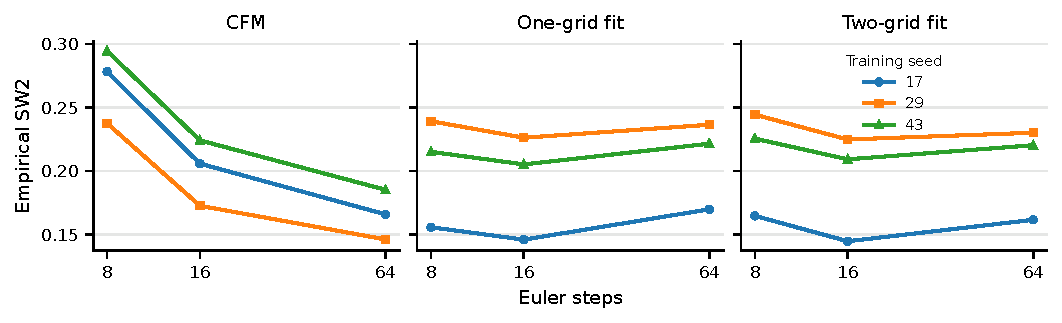
\includegraphics[width=.82\textwidth]{../results/large_bank/large_bank_d2.pdf}
\caption{Sliced Wasserstein distance (SW2) at 8, 16, and 64 Euler steps
on the 262,144-sample evaluation set. Each line is one trained field.
All nine distances decrease from 8 to 16 steps. At 64 steps, the
one-grid fields with seeds 17 and 43 have larger distances than at
8 steps.}
\label{fig:large-bank}
\end{figure}

All nine sliced distances decrease from eight to sixteen steps on this
evaluation set. Only the one-grid fields with seeds 17 and 43 increase from eight to 64 steps.
The direction of the change from 8 to 16 steps depends on the
evaluation set. The independent trigonometric
witness estimates agree with the preceding diagnostic to approximately
$5.1\times10^{-15}$. The witness metric and SW2 measure different properties of a distribution.
Their values and comparisons need not agree. They are not interchangeable
estimates of one metric.

To examine whether the shared sine/cosine form of training and diagnostic
features explains their behavior, we compare three dictionaries on the
same large evaluation set. They contain the 128 actual training features, 32
independently drawn sine/cosine features, and 32 independent functions
$\tanh(v_j^\top x-c_j)$ with $|v_j|\le1$ and $c_j\in[-2,2]$.
The last dictionary has bounded 1-Lipschitz functions and does not use
trigonometric features. We compare whether each dictionary's discrepancy increases or decreases.
The dictionaries contain different numbers and types of functions, so
their absolute values are not one common metric. For the six one-grid and two-grid fields,
both trigonometric dictionaries decrease from eight to sixteen steps.
The tanh dictionary decreases for five and increases for the one-grid field with
seed 29. Thus improvement is not confined to the shared trigonometric
form. This exploratory comparison neither establishes nor rules out a
causal training-feature preference. It adds no simultaneous confidence
claim beyond the preceding predeclared witness analysis.

\subsection{Analytical checks and global derivative bounds}
The deterministic controls check the formulas for equal refinements
$m=2,3,4$, the sharp scalar constant, degenerate splits, $N$ versus $N+1$,
equal-defect solver pairs, temporal aliasing, endpoint cancellation, and
conditional radial moments. Numerical integration checks radial moments
in selected examples. These calculations check the implementation, not the
general proof. The full inverse formula uses explicit Gaussian moments
and Hermite coefficients. Its floating-point evaluation is not an interval
certificate, and its high-degree constants can be numerically enormous.

Every fitted network has a sufficient global derivative bound established by
integer upper bounds on Frobenius norms of its exact stored binary
coefficients (Supplementary Section~\ref{app:network-budgets}). Across the 30 fitted fields,
these sufficient derivative bounds range from 12,096 to 50,688. They prove class
membership for the corresponding real tanh networks but are far too large
for a useful application of the worst-case risk thresholds. They are not
estimated local Jacobian norms or certificates for finite-precision inference.

Repetition of all 18 primary training runs in the same software environment
reproduced their parameter tensors and non-timing evaluation results.
Unit tests check finite computations; the analytical theorems rely on their
mathematical proofs.

\subsection{Population Wasserstein error on a three-dimensional mixture}
\label{app:population-example}
The target in Section~\ref{sec:population-example} is
$Y=\mu\xi e_1+\sigma Z$ with $\mu=1.5$, $\sigma=0.5$, symmetric sign
$\xi$, and independent standard Gaussian $Z$. Use the exact conditional
field \eqref{eq:mixture-generator}. In the second field, replace its
two Gaussian coordinates by the linear velocity $M'(t)M(t)^{-1}x$,
where $M(t)=(1-t)I_2+\sigma tJ$ and $J$ rotates the plane by a quarter
turn. This block has the same Gaussian marginals as the conditional
field. Its Euler update equals $M(t+h)M(t)^{-1}x$ because $M$ is affine
in time. Both fields obey a common finite derivative bound. The
mixture coordinate has the same velocity in both fields.

The exact and numerical laws each factor into a scalar law and a planar
Gaussian. Any pairing must pay at least the optimal squared cost in
each block. Since the blocks are independent, we can choose an optimal
pairing in each block and combine them. This attains the sum of the
two costs, so the squared Wasserstein distance adds across blocks.
In the plane, if the numerical and target coordinate standard deviations
are $s$ and $g(t)=\sqrt{(1-t)^2+\sigma^2t^2}$, the squared distance is
$2(s-g(t))^2$. For the skew field, this term is zero in exact arithmetic.

In the mixture coordinate, the spatial derivative of the nonlinear
velocity term is nonnegative on $[0,1]$. The spatial derivative of its linear term is
bounded below by $-(1+\sigma^2)/(2\sigma)=-1.25$. All tested Euler maps
are therefore increasing. Pair the numerical particle started from $z$
with the target point at cumulative probability $\Phi(z)$, where $\Phi$
is the standard Gaussian cumulative distribution function. This pairing
attains the scalar Wasserstein distance. Invert the two-component mixture
distribution by bisection. Integrate the squared distance against the
standard Gaussian density. Symmetry allows integration on $[0,9]$ with
twice the weight. The omitted squared tail is at most $1.07\times10^{-15}$.
To bound it, use $|X^{\mathrm{Euler}}|\le e^{1.25}(|z|+7.5)$ and the
target quantile bound $|Q_t(\Phi(z))|\le |z|+1.5$, then integrate the
square of their sum outside $[-9,9]$.

Doubling the Gauss--Legendre quadrature from 512 to 1,024 nodes changes
each reported error sum by less than $10^{-12}$ relative. The largest
relative residual in the quantile survival probabilities is below
$4\times10^{-14}$. The skew block agrees with the exact target standard
deviation within $7\times10^{-16}$. These are numerical checks on the
quadrature and floating-point arithmetic. The tail estimate is analytical.

Table~\ref{tab:population-example} gives the maxima over every shared
coarse node, separately for each run. The local order is
$\log_2(\mathcal J_{N/2}/\mathcal J_N)$. This example gives two observed
rates under the conditions of Theorem~\ref{thm:odd-transfer}. For these
fields, Theorem~\ref{thm:source-risk} also gives an obstruction. Here
$\nu=3$, and the initial excess loss $\Delta_0$ is zero for the
conditional field and $0.5$ for the skew field. Both differ from $\nu$,
so the error sum is at least of order $1/N$ for sufficiently fine grids.
Both fields generate the path exactly, so the standard Euler bound gives
an upper error of order $1/N$ on uniform grids.
The smaller error with the planar correction concerns this product path
and these two fields. The scalar optimum in Section~\ref{sec:sharpness}
concerns a different path and an optimization over fields.

\begin{table}[t]
\centering
\caption{Population $W_2$ errors for two exact generators of the three-dimensional mixture path. Errors are deterministic quadrature estimates, with no training or evaluation samples. Lower errors are better. Order is estimated from the sum of the errors at consecutive coarse step counts.}
\label{tab:population-example}
\small
\begin{tabular}{@{}r rrr rrr@{}}
\toprule
& \multicolumn{3}{c}{Conditional velocity} & \multicolumn{3}{c}{Planar skew}\\
$N$ & $E_c$ & $E_f$ & Order & $E_c$ & $E_f$ & Order\\
\midrule
8 & 0.1932745 & 0.0992033 & \multicolumn{1}{c}{--} & 0.1511015 & 0.0768981 & \multicolumn{1}{c}{--}\\
16 & 0.0992033 & 0.0503485 & 0.968 & 0.0768981 & 0.0388608 & 0.978\\
32 & 0.0503485 & 0.0253755 & 0.982 & 0.0388608 & 0.0195436 & 0.987\\
64 & 0.0253755 & 0.0127400 & 0.990 & 0.0195436 & 0.0098015 & 0.993\\
128 & 0.0127400 & 0.0063833 & 0.995 & 0.0098015 & 0.0049083 & 0.996\\
256 & 0.0063833 & 0.0031950 & 0.997 & 0.0049083 & 0.0024561 & 0.998\\
\bottomrule
\end{tabular}
\end{table}


\section{Learned scalar fields with population errors}
\label{app:scalar-population}
This section gives the training and evaluation methods for the scalar
fields of Section~\ref{sec:scalar-learned}. We estimate population
errors by numerical integration over a Gaussian start.\AIassistance

\subsection{Target, fields, and training}
The target is $Y=\mu\xi+\sigma Z$ with $\mu=1.5$, $\sigma=0.5$, a
symmetric random sign $\xi$, and an independent standard Gaussian $Z$.
The path is the independent interpolation \eqref{eq:independent}. Thus
$p_t$ is an equal mixture of the two Gaussians
$\mathcal N(\pm\mu t,(1-t)^2+\sigma^2t^2)$. The dimension is odd, so
Theorem~\ref{thm:odd-transfer} applies. The exact conditional velocity is
\eqref{eq:mixture-generator} with $d=1$.

Each field is a network with the input $(x,t)$, two hidden layers of 48
tanh units, and a scalar output. It has 2,545 parameters. The step size
is not an input. There are three objectives.
\begin{itemize}
\item \emph{CFM.} The conditional flow matching loss
$\E|u(t,(1-t)G+tY)-(Y-G)|^2$, with $t$ uniform on $[0,1]$ and a
minibatch of 1,024 independent draws.
\item \emph{One-grid fit.} The CFM loss plus $10\,L_8$.
\item \emph{Two-grid fit.} The CFM loss plus $10\,(L_8+L_{16})/2$.
\end{itemize}
The loss $L_n$ is computed as follows. Run $n$ uniform Euler steps from
1,024 new Gaussian start points. Take each of the times
$1/4,1/2,3/4,1$. Sort the Euler outputs and sort 1,024 new samples of
$p_t$. Then take the mean squared difference of the sorted values. This value is the squared
$W_2$ distance between the two empirical distributions. The loss $L_n$
is the mean over the four times, and its gradient is taken through the
Euler steps.

Each run uses 8,000 Adam updates with the learning rate $10^{-3}$ in
double precision. New samples are drawn at each update. Each objective
uses the ten seeds 0 to 9, which gives \ScalarModelCount{} fields. All
settings were fixed before the evaluation, and no field was selected
with the evaluation results.

\subsection{Population errors by quadrature}
Let $z\mapsto\widehat X_k(z)$ be the Euler map from the start point to
the state at node $k$. We evaluate it on 8,001 equally spaced points
$z\in[-9,9]$. If the map is increasing, the pairing of equal quantiles
is optimal, and
\[
 W_2^2(\Law(\widehat X_k),p_t)
 =\int\big(\widehat X_k(z)-Q_t(\Phi(z))\big)^2\varphi(z)\dd z .
\]
Here $Q_t$ is the quantile function of $p_t$, and $\Phi$ and $\varphi$
are the standard Gaussian distribution function and density. We compute
$Q_t$ by bisection on the distribution function of the mixture, and the
integral by the trapezoidal rule. The Gaussian mass outside $[-9,9]$ is
below $3\times10^{-19}$. For all \ScalarModelCount{} fields, the Euler maps increase on the
quadrature nodes. We also bound the derivative of each update,
$1+\partial_xu/N$, from the network weights. For $N=4,8,16$ we
propagate bounds through both layers on intervals covering the real
line. For $N\ge32$ we use the sum of the negative products of weights
along paths from the input to the output. Each tanh derivative lies
between zero and one. The smallest computed lower bound is above
$0.037$. These checks use double precision without directed rounding. For the exact conditional
velocity, this quadrature gives the skew-field columns of
Table~\ref{tab:population-example}, which contain only the error in the mixture
coordinate, to seven digits.

The reference for the exact flow of a field is the classical
fourth-order Runge--Kutta method with 1,024 steps. The \emph{model bias}
is the largest $W_2$ distance between this reference and the target path
at 64 equally spaced times. The \emph{integration error} at $N$ steps compares the
Euler run and the reference from the same start points. It is their
largest root mean squared distance at the four shared times. The
\emph{target error} at $N$ steps is the largest $W_2$ distance to the
target path at the four shared times. The quantities $E_c$ and $E_f$ of
\eqref{eq:errors} use all nodes of the coarse grid.

\subsection{Results}
Table~\ref{tab:scalar-models} gives the results for each field. The
means are in Table~\ref{tab:scalar} of the main article.

\emph{CFM fields.} The target error is smaller at 16, 64, and 256 steps
than at 8 steps for all ten seeds. The mean is \ScalarCfmEight{} at 8
steps and \ScalarCfmLarge{} at 256 steps. The model bias is between
\ScalarCfmBiasMin{} and \ScalarCfmBiasMax{}, with a mean of
\ScalarCfmBias{}. For \ScalarCfmArgminLast{} of the ten seeds, the
smallest target error is at 256 steps. For the other seeds it is at an
intermediate step count, and the difference from the value at 256 steps
is small.

\emph{One-grid fields.} The mean target error is \ScalarOneEight{} at 8
steps, \ScalarOneSixteen{} at 16 steps, \ScalarOneSixtyFour{} at 64
steps, and \ScalarOneLarge{} at 256 steps. The smallest target error is
at 8 steps for \ScalarOneArgminEight{} seeds and at 16 steps for
\ScalarOneArgminSixteen{} seeds. Compare each value with the value
at 8 steps. The target error is larger at 16 steps for
\ScalarOneIncreaseSixteen{} of the ten seeds, at 64 steps for
\ScalarOneIncreaseSixtyFour{} seeds, and at 256 steps for
\ScalarOneIncreaseLarge{} seeds. The exact two-sided
Wilcoxon signed-rank tests for these three paired comparisons give
$p=\ScalarOneWilcoxonSixteen$, $p=\ScalarOneWilcoxonSixtyFour$, and
$p=\ScalarOneWilcoxonLarge$. The mean model bias is \ScalarOneBias{}.
The mean integration error decreases from \ScalarOneOwnEight{} at 8
steps to \ScalarOneOwnLarge{} at 256 steps.

\emph{Two-grid fields.} The mean target error is \ScalarTwoEight{} at 8
steps, \ScalarTwoSixteen{} at 16 steps, \ScalarTwoSixtyFour{} at 64
steps, and \ScalarTwoLarge{} at 256 steps. The smallest target error is
at 16 steps for \ScalarTwoArgminSixteen{} of the ten seeds. Compared
with the value at 8 steps, the target error is larger at 64 steps for
\ScalarTwoIncreaseSixtyFour{} seeds and at 256 steps for
\ScalarTwoIncreaseLarge{} seeds ($p=\ScalarTwoWilcoxonSixtyFour$ and
$p=\ScalarTwoWilcoxonLarge$). Compared with the value at 16 steps, it
is larger at 64 steps for \ScalarTwoFromSixteenIncreaseSixtyFour{} seeds
and at 256 steps for \ScalarTwoFromSixteenIncreaseLarge{} seeds
($p=\ScalarTwoFromSixteenWilcoxonSixtyFour$ and
$p=\ScalarTwoFromSixteenWilcoxonLarge$). The same comparison with the
value at 16 steps gives \ScalarOneFromSixteenIncreaseSixtyFour{} and
\ScalarOneFromSixteenIncreaseLarge{} seeds for the one-grid fields, and
\ScalarCfmFromSixteenIncreaseSixtyFour{} and
\ScalarCfmFromSixteenIncreaseLarge{} seeds for the CFM fields. The mean
model bias of the two-grid fields is \ScalarTwoBias{}.

For a fixed field, the target error at the four evaluation times
approaches the bias over those times as the step count increases. The
theoretical two-grid error uses all shared nodes and approaches twice
the bias over the full time interval. The table gives a 64-time estimate
of bias and the two-grid error at $N=8$. Theorem~\ref{thm:characterization}
concerns the best error over a class of fields. A fit at small step counts
decreases the target error there. For the one-grid fields it also
increases the model bias. The weight of the added loss was fixed and
was not tuned, and a different weight can change the size of the
effect.

\begin{table}[ht]
\centering
\caption{Learned scalar fields: target error at $N$ Euler steps for each
field, model bias, and the two-grid error $E_c+E_f$ of \eqref{eq:errors}
at $N=8$. All values are population $W_2$ distances computed by
quadrature.}
\label{tab:scalar-models}
\begin{tabular}{@{}lrcccccc@{}}
\toprule
Field & Seed & $N=8$ & $16$ & $64$ & $256$ & Model bias & $E_c+E_f$ at $N=8$\\
\midrule
CFM & 0 & 0.146 & 0.072 & 0.025 & 0.021 & 0.023 & 0.218\\
CFM & 1 & 0.150 & 0.097 & 0.089 & 0.093 & 0.094 & 0.247\\
CFM & 2 & 0.143 & 0.078 & 0.050 & 0.051 & 0.052 & 0.220\\
CFM & 3 & 0.174 & 0.119 & 0.101 & 0.102 & 0.102 & 0.293\\
CFM & 4 & 0.148 & 0.076 & 0.040 & 0.040 & 0.041 & 0.225\\
CFM & 5 & 0.137 & 0.067 & 0.040 & 0.044 & 0.046 & 0.204\\
CFM & 6 & 0.257 & 0.217 & 0.198 & 0.196 & 0.195 & 0.473\\
CFM & 7 & 0.234 & 0.196 & 0.186 & 0.186 & 0.187 & 0.430\\
CFM & 8 & 0.187 & 0.143 & 0.131 & 0.132 & 0.133 & 0.330\\
CFM & 9 & 0.161 & 0.089 & 0.045 & 0.039 & 0.039 & 0.251\\
\addlinespace
One-grid fit & 0 & 0.073 & 0.079 & 0.110 & 0.119 & 0.123 & 0.152\\
One-grid fit & 1 & 0.068 & 0.068 & 0.099 & 0.108 & 0.112 & 0.136\\
One-grid fit & 2 & 0.088 & 0.090 & 0.114 & 0.122 & 0.125 & 0.178\\
One-grid fit & 3 & 0.107 & 0.112 & 0.138 & 0.147 & 0.150 & 0.219\\
One-grid fit & 4 & 0.122 & 0.129 & 0.151 & 0.159 & 0.161 & 0.251\\
One-grid fit & 5 & 0.168 & 0.169 & 0.185 & 0.191 & 0.193 & 0.336\\
One-grid fit & 6 & 0.065 & 0.041 & 0.068 & 0.078 & 0.084 & 0.106\\
One-grid fit & 7 & 0.055 & 0.047 & 0.082 & 0.092 & 0.096 & 0.102\\
One-grid fit & 8 & 0.053 & 0.049 & 0.084 & 0.094 & 0.098 & 0.102\\
One-grid fit & 9 & 0.048 & 0.057 & 0.096 & 0.107 & 0.110 & 0.105\\
\addlinespace
Two-grid fit & 0 & 0.091 & 0.090 & 0.114 & 0.122 & 0.125 & 0.181\\
Two-grid fit & 1 & 0.100 & 0.091 & 0.110 & 0.117 & 0.120 & 0.191\\
Two-grid fit & 2 & 0.112 & 0.103 & 0.119 & 0.125 & 0.127 & 0.215\\
Two-grid fit & 3 & 0.107 & 0.073 & 0.079 & 0.085 & 0.088 & 0.180\\
Two-grid fit & 4 & 0.103 & 0.092 & 0.109 & 0.116 & 0.118 & 0.196\\
Two-grid fit & 5 & 0.079 & 0.050 & 0.070 & 0.079 & 0.082 & 0.129\\
Two-grid fit & 6 & 0.086 & 0.064 & 0.081 & 0.088 & 0.091 & 0.150\\
Two-grid fit & 7 & 0.077 & 0.041 & 0.059 & 0.068 & 0.073 & 0.117\\
Two-grid fit & 8 & 0.089 & 0.048 & 0.053 & 0.059 & 0.062 & 0.137\\
Two-grid fit & 9 & 0.078 & 0.039 & 0.057 & 0.067 & 0.071 & 0.117\\
\bottomrule
\end{tabular}

\end{table}

\section{Variability of sample-based comparisons across evaluation sets}
\label{app:set-variability}
Section~\ref{app:experiments} reports the sliced distance SW2 on one
evaluation set of 1,024 samples and on one evaluation set of 262,144
samples. The two sets give different directions for the change between
8 and 16 steps. Here we measure how often the direction changes across
independent evaluation sets of the same size.\AIassistance

\subsection{Protocol}
The nine two-dimensional fields of Section~\ref{app:experiments} and its
128 projection directions are fixed. Only
the evaluation samples change. One evaluation set contains start points
for the numerical runs, and independent noise and data points for the
target path. We draw \VarSmallSets{} independent sets of 1,024 samples and
\VarMediumSets{} independent sets of 16,384 samples. Their random seeds are different from the seeds of
those two sets. For each set we compute SW2 at 8, 16, and 64 Euler steps
as the maximum over the five diagnostic times, in double precision.
This implementation gives the values of Table~\ref{tab:seed-grid-details} on
the separate 1,024-sample set with differences below $3\times10^{-8}$.

\subsection{Results}
Table~\ref{tab:set-variability} gives the results for each field and
each size. It gives the mean and the standard deviation across sets of
SW2, of its change from 8 to 16 steps, and of its change from 8 to 64
steps. It also gives the percentage
of sets in which SW2 increases.

\emph{Change from 8 to 16 steps.} For the three CFM fields, SW2 decreases in all sets of both sizes. For the six fitted fields (one-grid fit and two-grid
fit), the mean change is negative at both sizes. With
1,024 samples, the standard deviation of the change across sets is
\VarSmallChangeSd{} on average over the six fields, and the mean change
is $\VarSmallChangeMean$. SW2 increases in \VarSmallFractionMin{}\% to
\VarSmallFractionMax{}\% of the sets, as a function of the field. At
least one of the six fields shows an increase in \VarSmallAnySix{}\% of
the sets, and all six fields show an increase together in
\VarSmallAllSix{}\% of the sets. The separate 1,024-sample set also shows all six increases. With 16,384 samples, the standard deviation of the
change is \VarMediumChangeSd{}, and SW2 increases in at most
\VarMediumFractionMax{}\% of the sets. On the set of 262,144
samples, SW2 decreases for all six fields
(Table~\ref{tab:large-bank}).

\emph{Change from 8 to 64 steps.} This change differs between the
fields. For the one-grid field with seed 17, the mean change is positive at both sizes. SW2 increases in \VarSmallGridLongFraction{}\% of the
sets of 1,024 samples and in \VarMediumGridLongFraction{}\% of the sets
of 16,384 samples. It also increases on the set of 262,144
samples. This agrees with the finite-witness intervals of
Section~\ref{app:large-bank-timing} for the same field. With 16,384
samples, the values for the other two one-grid fields are
\VarMediumLongOneB{}\% and \VarMediumLongOneC{}\%, and the values for
the three two-grid fields are \VarMediumLongTwoA{}\%,
\VarMediumLongTwoB{}\%, and \VarMediumLongTwoC{}\%.

With these fields and directions, increases from 8 to 16 steps occur
less often on sets of 16,384 samples than on sets of 1,024. The same
samples are used across fields within a set, so changes for the six
fields are correlated. The mean SW2 values in
Table~\ref{tab:set-variability} are also smaller on the larger sets.

\begin{table*}[ht]
\centering
\caption{Empirical SW2 of the nine two-dimensional fields on independent
evaluation sets. Entries are means across sets, with standard deviations
across sets in parentheses. The two increase columns give the percentages of sets in which SW2
increases from 8 to 16 and from 8 to 64 steps.}
\label{tab:set-variability}
\footnotesize
\begin{tabular}{@{}llrccccccc@{}}
\toprule
Training & Seed & Set size & SW2$_8$ & SW2$_{16}$ & SW2$_{64}$ & Change 8 to 16 & Increase & Change 8 to 64 & Increase\\
\midrule
CFM & 17 & 1,024 & 0.305 (0.029) & 0.243 (0.034) & 0.213 (0.040) & $-0.062$ (0.011) & 0\% & $-0.092$ (0.022) & 0\%\\
CFM & 17 & 16,384 & 0.280 (0.006) & 0.208 (0.006) & 0.169 (0.008) & $-0.072$ (0.003) & 0\% & $-0.111$ (0.007) & 0\%\\
\addlinespace
CFM & 29 & 1,024 & 0.266 (0.042) & 0.212 (0.049) & 0.193 (0.053) & $-0.054$ (0.014) & 0\% & $-0.073$ (0.026) & 0\%\\
CFM & 29 & 16,384 & 0.241 (0.012) & 0.177 (0.015) & 0.152 (0.018) & $-0.063$ (0.005) & 0\% & $-0.089$ (0.011) & 0\%\\
\addlinespace
CFM & 43 & 1,024 & 0.315 (0.042) & 0.251 (0.050) & 0.218 (0.056) & $-0.064$ (0.012) & 0\% & $-0.097$ (0.023) & 0\%\\
CFM & 43 & 16,384 & 0.297 (0.010) & 0.228 (0.012) & 0.189 (0.015) & $-0.070$ (0.004) & 0\% & $-0.108$ (0.008) & 0\%\\
\addlinespace
One-grid fit & 17 & 1,024 & 0.206 (0.050) & 0.201 (0.055) & 0.221 (0.056) & $-0.005$ (0.014) & 38\% & $+0.016$ (0.023) & 74\%\\
One-grid fit & 17 & 16,384 & 0.157 (0.014) & 0.147 (0.015) & 0.171 (0.014) & $-0.010$ (0.005) & 7\% & $+0.014$ (0.008) & 100\%\\
\addlinespace
One-grid fit & 29 & 1,024 & 0.260 (0.069) & 0.248 (0.073) & 0.259 (0.071) & $-0.012$ (0.012) & 18\% & $-0.001$ (0.020) & 48\%\\
One-grid fit & 29 & 16,384 & 0.244 (0.018) & 0.231 (0.020) & 0.241 (0.020) & $-0.013$ (0.004) & 0\% & $-0.003$ (0.007) & 30\%\\
\addlinespace
One-grid fit & 43 & 1,024 & 0.253 (0.054) & 0.246 (0.063) & 0.261 (0.067) & $-0.007$ (0.014) & 31\% & $+0.008$ (0.022) & 65\%\\
One-grid fit & 43 & 16,384 & 0.213 (0.011) & 0.202 (0.015) & 0.218 (0.016) & $-0.011$ (0.004) & 0\% & $+0.006$ (0.007) & 77\%\\
\addlinespace
Two-grid fit & 17 & 1,024 & 0.212 (0.048) & 0.199 (0.054) & 0.214 (0.056) & $-0.013$ (0.015) & 20\% & $+0.002$ (0.024) & 58\%\\
Two-grid fit & 17 & 16,384 & 0.166 (0.013) & 0.146 (0.015) & 0.163 (0.015) & $-0.020$ (0.005) & 0\% & $-0.003$ (0.008) & 33\%\\
\addlinespace
Two-grid fit & 29 & 1,024 & 0.265 (0.067) & 0.247 (0.072) & 0.253 (0.071) & $-0.018$ (0.012) & 6\% & $-0.012$ (0.020) & 29\%\\
Two-grid fit & 29 & 16,384 & 0.249 (0.018) & 0.230 (0.020) & 0.235 (0.020) & $-0.019$ (0.004) & 0\% & $-0.014$ (0.007) & 7\%\\
\addlinespace
Two-grid fit & 43 & 1,024 & 0.262 (0.053) & 0.248 (0.063) & 0.259 (0.068) & $-0.013$ (0.014) & 20\% & $-0.003$ (0.023) & 50\%\\
Two-grid fit & 43 & 16,384 & 0.223 (0.011) & 0.206 (0.014) & 0.217 (0.016) & $-0.017$ (0.005) & 0\% & $-0.006$ (0.007) & 20\%\\
\bottomrule
\end{tabular}

\end{table*}

\section*{Acknowledgment of AI Assistance}
OpenAI models GPT-5.6 Sol and GPT-6 Astra
assisted substantially with mathematical analysis, proof verification,
experimental code, figures, and writing in Supplementary Sections~S1--S14~\citep{openai_chatgpt,openai_codex}. OpenAI Codex, with the model
GPT-6.1 Sol, assisted with writing and experimental code in these sections~\citep{openai_codex}. Anthropic Claude Fable 5.2 assisted
with writing, mathematical analysis, numerical verification, and the
experiments of Supplementary
Sections~\ref{app:scalar-population} and~\ref{app:set-variability}~\citep{anthropic_claude_fable}.
The author takes responsibility for the scientific content and
attribution.
\bibliographystyle{IEEEtran}
\bibliography{supplement-references}
\end{document}
